% Generated by scripts/latex-perf-book.mjs. Do not edit by hand.
\documentclass[11pt]{article}
\usepackage{fontspec}
\setmainfont{Latin Modern Roman}
\usepackage{amsmath,amssymb}
\usepackage{booktabs}
\usepackage{graphicx}
\usepackage[margin=2.5cm]{geometry}
\usepackage{microtype}
\usepackage{hyperref}

\title{MDraft LaTeX performance: book multi-file}
\author{MDraft benchmarks}
\date{}

\begin{document}
\maketitle
\tableofcontents

\section{Introduction}
\label{sec:intro}

Performance probe paragraph M0. This project is the large case in MDraft's
LuaLaTeX benchmark. It has a main file, twelve included chapters, valid
equations, tables, cross-chapter references, a local image and a bibliography.
The benchmark edits the main file and the included chapters and checks that the
preview still renders the whole project.

The first chapter equation is Equation~\ref{eq:ch01:integral}; the last chapter
table is Table~\ref{tab:ch12:runs}. The image is Figure~\ref{fig:main:diagram}.
The bibliography includes \cite{knuth1984} and \cite{lamport1994}.

\begin{figure}[h]
  \centering
  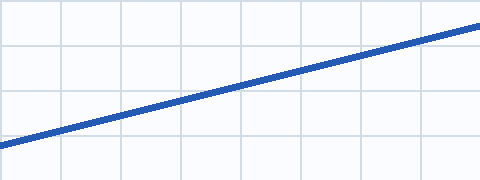
\includegraphics[width=0.45\linewidth]{figures/diagram.png}
  \caption{A local image used by the benchmark.}
  \label{fig:main:diagram}
\end{figure}

% Generated by scripts/latex-perf-book.mjs. Do not edit by hand.
\section{Chapter 1: Baseline}
\label{sec:ch01}

Performance probe paragraph B01. This is included chapter 1 of twelve in
the large MDraft LuaLaTeX benchmark. Ordinary prose keeps the page count
realistic and gives the probe a stable word to edit. Equation~\ref{eq:ch12:integral} and
Table~\ref{tab:ch12:runs} are valid cross-chapter references.

\subsection{An integral}
The integral in Equation~\ref{eq:ch01:integral} is valid for every integer
$n \ge 0$. It is deliberately simple; the benchmark measures the engine, not
the mathematics.

\begin{equation}
  \label{eq:ch01:integral}
  \int_{0}^{1} x^{n}\,dx = \frac{1}{n+1}.
\end{equation}

The geometric series in Equation~\ref{eq:ch01:series} converges for
$|r| < 1$ and gives a second display to render in this chapter.

\begin{equation}
  \label{eq:ch01:series}
  \sum_{k=0}^{m} r^{k} = \frac{1-r^{m+1}}{1-r}.
\end{equation}

\subsection{A table}
\begin{table}[h]
  \centering
  \begin{tabular}{lrr}
    \toprule
    Run & Time & Pages \\
    \midrule
    One   & 1.20 & 3 \\
    Two   & 1.15 & 3 \\
    Three & 1.18 & 3 \\
    \bottomrule
  \end{tabular}
  \caption{A timing sample for chapter 1.}
  \label{tab:ch01:runs}
\end{table}

Table~\ref{tab:ch01:runs} is a valid float with a caption and a label. It
exists so the page builder has a boxed object that cannot be split across a
page break. The bibliography entry \cite{knuth1984} is resolved by the same compile.

\subsection{More prose}
A benchmark chapter needs enough text that the type\-set is visible above the
engine boot. This paragraph, the next one and the table above add up to a few
pages per chapter.

The content is intentionally repetitive across chapters. The point is not the
prose; it is that the include graph, the equation numbering and the table
labels all have to stay consistent while the probe edits one letter.

The final paragraph of chapter 1 gives the probe a second stable offset. A
change here must not invalidate the labels in any other chapter.

\subsection{Part 2}

This is included chapter 1 of twelve in
the large MDraft LuaLaTeX benchmark. Ordinary prose keeps the page count
realistic and gives the probe a stable word to edit. Equation~\ref{eq:ch12:k2:integral} and
Table~\ref{tab:ch12:k2:runs} are valid cross-chapter references.

\subsubsection{An integral}
The integral in Equation~\ref{eq:ch01:k2:integral} is valid for every integer
$n \ge 0$. It is deliberately simple; the benchmark measures the engine, not
the mathematics.

\begin{equation}
  \label{eq:ch01:k2:integral}
  \int_{0}^{1} x^{n}\,dx = \frac{1}{n+1}.
\end{equation}

The geometric series in Equation~\ref{eq:ch01:k2:series} converges for
$|r| < 1$ and gives a second display to render in this chapter.

\begin{equation}
  \label{eq:ch01:k2:series}
  \sum_{k=0}^{m} r^{k} = \frac{1-r^{m+1}}{1-r}.
\end{equation}

\subsubsection{A table}
\begin{table}[h]
  \centering
  \begin{tabular}{lrr}
    \toprule
    Run & Time & Pages \\
    \midrule
    One   & 1.20 & 3 \\
    Two   & 1.15 & 3 \\
    Three & 1.18 & 3 \\
    \bottomrule
  \end{tabular}
  \caption{A timing sample for chapter 1.}
  \label{tab:ch01:k2:runs}
\end{table}

Table~\ref{tab:ch01:k2:runs} is a valid float with a caption and a label. It
exists so the page builder has a boxed object that cannot be split across a
page break. The bibliography entry \cite{knuth1984} is resolved by the same compile.

\subsubsection{More prose}
A benchmark chapter needs enough text that the type\-set is visible above the
engine boot. This paragraph, the next one and the table above add up to a few
pages per chapter.

The content is intentionally repetitive across chapters. The point is not the
prose; it is that the include graph, the equation numbering and the table
labels all have to stay consistent while the probe edits one letter.

The final paragraph of chapter 1 gives the probe a second stable offset. A
change here must not invalidate the labels in any other chapter.

\subsection{Part 3}

This is included chapter 1 of twelve in
the large MDraft LuaLaTeX benchmark. Ordinary prose keeps the page count
realistic and gives the probe a stable word to edit. Equation~\ref{eq:ch12:k3:integral} and
Table~\ref{tab:ch12:k3:runs} are valid cross-chapter references.

\subsubsection{An integral}
The integral in Equation~\ref{eq:ch01:k3:integral} is valid for every integer
$n \ge 0$. It is deliberately simple; the benchmark measures the engine, not
the mathematics.

\begin{equation}
  \label{eq:ch01:k3:integral}
  \int_{0}^{1} x^{n}\,dx = \frac{1}{n+1}.
\end{equation}

The geometric series in Equation~\ref{eq:ch01:k3:series} converges for
$|r| < 1$ and gives a second display to render in this chapter.

\begin{equation}
  \label{eq:ch01:k3:series}
  \sum_{k=0}^{m} r^{k} = \frac{1-r^{m+1}}{1-r}.
\end{equation}

\subsubsection{A table}
\begin{table}[h]
  \centering
  \begin{tabular}{lrr}
    \toprule
    Run & Time & Pages \\
    \midrule
    One   & 1.20 & 3 \\
    Two   & 1.15 & 3 \\
    Three & 1.18 & 3 \\
    \bottomrule
  \end{tabular}
  \caption{A timing sample for chapter 1.}
  \label{tab:ch01:k3:runs}
\end{table}

Table~\ref{tab:ch01:k3:runs} is a valid float with a caption and a label. It
exists so the page builder has a boxed object that cannot be split across a
page break. The bibliography entry \cite{knuth1984} is resolved by the same compile.

\subsubsection{More prose}
A benchmark chapter needs enough text that the type\-set is visible above the
engine boot. This paragraph, the next one and the table above add up to a few
pages per chapter.

The content is intentionally repetitive across chapters. The point is not the
prose; it is that the include graph, the equation numbering and the table
labels all have to stay consistent while the probe edits one letter.

The final paragraph of chapter 1 gives the probe a second stable offset. A
change here must not invalidate the labels in any other chapter.

\subsection{Part 4}

This is included chapter 1 of twelve in
the large MDraft LuaLaTeX benchmark. Ordinary prose keeps the page count
realistic and gives the probe a stable word to edit. Equation~\ref{eq:ch12:k4:integral} and
Table~\ref{tab:ch12:k4:runs} are valid cross-chapter references.

\subsubsection{An integral}
The integral in Equation~\ref{eq:ch01:k4:integral} is valid for every integer
$n \ge 0$. It is deliberately simple; the benchmark measures the engine, not
the mathematics.

\begin{equation}
  \label{eq:ch01:k4:integral}
  \int_{0}^{1} x^{n}\,dx = \frac{1}{n+1}.
\end{equation}

The geometric series in Equation~\ref{eq:ch01:k4:series} converges for
$|r| < 1$ and gives a second display to render in this chapter.

\begin{equation}
  \label{eq:ch01:k4:series}
  \sum_{k=0}^{m} r^{k} = \frac{1-r^{m+1}}{1-r}.
\end{equation}

\subsubsection{A table}
\begin{table}[h]
  \centering
  \begin{tabular}{lrr}
    \toprule
    Run & Time & Pages \\
    \midrule
    One   & 1.20 & 3 \\
    Two   & 1.15 & 3 \\
    Three & 1.18 & 3 \\
    \bottomrule
  \end{tabular}
  \caption{A timing sample for chapter 1.}
  \label{tab:ch01:k4:runs}
\end{table}

Table~\ref{tab:ch01:k4:runs} is a valid float with a caption and a label. It
exists so the page builder has a boxed object that cannot be split across a
page break. The bibliography entry \cite{knuth1984} is resolved by the same compile.

\subsubsection{More prose}
A benchmark chapter needs enough text that the type\-set is visible above the
engine boot. This paragraph, the next one and the table above add up to a few
pages per chapter.

The content is intentionally repetitive across chapters. The point is not the
prose; it is that the include graph, the equation numbering and the table
labels all have to stay consistent while the probe edits one letter.

The final paragraph of chapter 1 gives the probe a second stable offset. A
change here must not invalidate the labels in any other chapter.

\subsection{Part 5}

This is included chapter 1 of twelve in
the large MDraft LuaLaTeX benchmark. Ordinary prose keeps the page count
realistic and gives the probe a stable word to edit. Equation~\ref{eq:ch12:k5:integral} and
Table~\ref{tab:ch12:k5:runs} are valid cross-chapter references.

\subsubsection{An integral}
The integral in Equation~\ref{eq:ch01:k5:integral} is valid for every integer
$n \ge 0$. It is deliberately simple; the benchmark measures the engine, not
the mathematics.

\begin{equation}
  \label{eq:ch01:k5:integral}
  \int_{0}^{1} x^{n}\,dx = \frac{1}{n+1}.
\end{equation}

The geometric series in Equation~\ref{eq:ch01:k5:series} converges for
$|r| < 1$ and gives a second display to render in this chapter.

\begin{equation}
  \label{eq:ch01:k5:series}
  \sum_{k=0}^{m} r^{k} = \frac{1-r^{m+1}}{1-r}.
\end{equation}

\subsubsection{A table}
\begin{table}[h]
  \centering
  \begin{tabular}{lrr}
    \toprule
    Run & Time & Pages \\
    \midrule
    One   & 1.20 & 3 \\
    Two   & 1.15 & 3 \\
    Three & 1.18 & 3 \\
    \bottomrule
  \end{tabular}
  \caption{A timing sample for chapter 1.}
  \label{tab:ch01:k5:runs}
\end{table}

Table~\ref{tab:ch01:k5:runs} is a valid float with a caption and a label. It
exists so the page builder has a boxed object that cannot be split across a
page break. The bibliography entry \cite{knuth1984} is resolved by the same compile.

\subsubsection{More prose}
A benchmark chapter needs enough text that the type\-set is visible above the
engine boot. This paragraph, the next one and the table above add up to a few
pages per chapter.

The content is intentionally repetitive across chapters. The point is not the
prose; it is that the include graph, the equation numbering and the table
labels all have to stay consistent while the probe edits one letter.

The final paragraph of chapter 1 gives the probe a second stable offset. A
change here must not invalidate the labels in any other chapter.

\subsection{Part 6}

This is included chapter 1 of twelve in
the large MDraft LuaLaTeX benchmark. Ordinary prose keeps the page count
realistic and gives the probe a stable word to edit. Equation~\ref{eq:ch12:k6:integral} and
Table~\ref{tab:ch12:k6:runs} are valid cross-chapter references.

\subsubsection{An integral}
The integral in Equation~\ref{eq:ch01:k6:integral} is valid for every integer
$n \ge 0$. It is deliberately simple; the benchmark measures the engine, not
the mathematics.

\begin{equation}
  \label{eq:ch01:k6:integral}
  \int_{0}^{1} x^{n}\,dx = \frac{1}{n+1}.
\end{equation}

The geometric series in Equation~\ref{eq:ch01:k6:series} converges for
$|r| < 1$ and gives a second display to render in this chapter.

\begin{equation}
  \label{eq:ch01:k6:series}
  \sum_{k=0}^{m} r^{k} = \frac{1-r^{m+1}}{1-r}.
\end{equation}

\subsubsection{A table}
\begin{table}[h]
  \centering
  \begin{tabular}{lrr}
    \toprule
    Run & Time & Pages \\
    \midrule
    One   & 1.20 & 3 \\
    Two   & 1.15 & 3 \\
    Three & 1.18 & 3 \\
    \bottomrule
  \end{tabular}
  \caption{A timing sample for chapter 1.}
  \label{tab:ch01:k6:runs}
\end{table}

Table~\ref{tab:ch01:k6:runs} is a valid float with a caption and a label. It
exists so the page builder has a boxed object that cannot be split across a
page break. The bibliography entry \cite{knuth1984} is resolved by the same compile.

\subsubsection{More prose}
A benchmark chapter needs enough text that the type\-set is visible above the
engine boot. This paragraph, the next one and the table above add up to a few
pages per chapter.

The content is intentionally repetitive across chapters. The point is not the
prose; it is that the include graph, the equation numbering and the table
labels all have to stay consistent while the probe edits one letter.

The final paragraph of chapter 1 gives the probe a second stable offset. A
change here must not invalidate the labels in any other chapter.

\subsection{Part 7}

This is included chapter 1 of twelve in
the large MDraft LuaLaTeX benchmark. Ordinary prose keeps the page count
realistic and gives the probe a stable word to edit. Equation~\ref{eq:ch12:k7:integral} and
Table~\ref{tab:ch12:k7:runs} are valid cross-chapter references.

\subsubsection{An integral}
The integral in Equation~\ref{eq:ch01:k7:integral} is valid for every integer
$n \ge 0$. It is deliberately simple; the benchmark measures the engine, not
the mathematics.

\begin{equation}
  \label{eq:ch01:k7:integral}
  \int_{0}^{1} x^{n}\,dx = \frac{1}{n+1}.
\end{equation}

The geometric series in Equation~\ref{eq:ch01:k7:series} converges for
$|r| < 1$ and gives a second display to render in this chapter.

\begin{equation}
  \label{eq:ch01:k7:series}
  \sum_{k=0}^{m} r^{k} = \frac{1-r^{m+1}}{1-r}.
\end{equation}

\subsubsection{A table}
\begin{table}[h]
  \centering
  \begin{tabular}{lrr}
    \toprule
    Run & Time & Pages \\
    \midrule
    One   & 1.20 & 3 \\
    Two   & 1.15 & 3 \\
    Three & 1.18 & 3 \\
    \bottomrule
  \end{tabular}
  \caption{A timing sample for chapter 1.}
  \label{tab:ch01:k7:runs}
\end{table}

Table~\ref{tab:ch01:k7:runs} is a valid float with a caption and a label. It
exists so the page builder has a boxed object that cannot be split across a
page break. The bibliography entry \cite{knuth1984} is resolved by the same compile.

\subsubsection{More prose}
A benchmark chapter needs enough text that the type\-set is visible above the
engine boot. This paragraph, the next one and the table above add up to a few
pages per chapter.

The content is intentionally repetitive across chapters. The point is not the
prose; it is that the include graph, the equation numbering and the table
labels all have to stay consistent while the probe edits one letter.

The final paragraph of chapter 1 gives the probe a second stable offset. A
change here must not invalidate the labels in any other chapter.

\subsection{Part 8}

This is included chapter 1 of twelve in
the large MDraft LuaLaTeX benchmark. Ordinary prose keeps the page count
realistic and gives the probe a stable word to edit. Equation~\ref{eq:ch12:k8:integral} and
Table~\ref{tab:ch12:k8:runs} are valid cross-chapter references.

\subsubsection{An integral}
The integral in Equation~\ref{eq:ch01:k8:integral} is valid for every integer
$n \ge 0$. It is deliberately simple; the benchmark measures the engine, not
the mathematics.

\begin{equation}
  \label{eq:ch01:k8:integral}
  \int_{0}^{1} x^{n}\,dx = \frac{1}{n+1}.
\end{equation}

The geometric series in Equation~\ref{eq:ch01:k8:series} converges for
$|r| < 1$ and gives a second display to render in this chapter.

\begin{equation}
  \label{eq:ch01:k8:series}
  \sum_{k=0}^{m} r^{k} = \frac{1-r^{m+1}}{1-r}.
\end{equation}

\subsubsection{A table}
\begin{table}[h]
  \centering
  \begin{tabular}{lrr}
    \toprule
    Run & Time & Pages \\
    \midrule
    One   & 1.20 & 3 \\
    Two   & 1.15 & 3 \\
    Three & 1.18 & 3 \\
    \bottomrule
  \end{tabular}
  \caption{A timing sample for chapter 1.}
  \label{tab:ch01:k8:runs}
\end{table}

Table~\ref{tab:ch01:k8:runs} is a valid float with a caption and a label. It
exists so the page builder has a boxed object that cannot be split across a
page break. The bibliography entry \cite{knuth1984} is resolved by the same compile.

\subsubsection{More prose}
A benchmark chapter needs enough text that the type\-set is visible above the
engine boot. This paragraph, the next one and the table above add up to a few
pages per chapter.

The content is intentionally repetitive across chapters. The point is not the
prose; it is that the include graph, the equation numbering and the table
labels all have to stay consistent while the probe edits one letter.

The final paragraph of chapter 1 gives the probe a second stable offset. A
change here must not invalidate the labels in any other chapter.

% Generated by scripts/latex-perf-book.mjs. Do not edit by hand.
\section{Chapter 2: Measurements}
\label{sec:ch02}

Performance probe paragraph B02. This is included chapter 2 of twelve in
the large MDraft LuaLaTeX benchmark. Ordinary prose keeps the page count
realistic and gives the probe a stable word to edit. Equation~\ref{eq:ch01:integral} and
Table~\ref{tab:ch01:runs} are valid cross-chapter references.

\subsection{An integral}
The integral in Equation~\ref{eq:ch02:integral} is valid for every integer
$n \ge 0$. It is deliberately simple; the benchmark measures the engine, not
the mathematics.

\begin{equation}
  \label{eq:ch02:integral}
  \int_{0}^{1} x^{n}\,dx = \frac{1}{n+1}.
\end{equation}

The geometric series in Equation~\ref{eq:ch02:series} converges for
$|r| < 1$ and gives a second display to render in this chapter.

\begin{equation}
  \label{eq:ch02:series}
  \sum_{k=0}^{m} r^{k} = \frac{1-r^{m+1}}{1-r}.
\end{equation}

\subsection{A table}
\begin{table}[h]
  \centering
  \begin{tabular}{lrr}
    \toprule
    Run & Time & Pages \\
    \midrule
    One   & 1.20 & 3 \\
    Two   & 1.15 & 3 \\
    Three & 1.18 & 3 \\
    \bottomrule
  \end{tabular}
  \caption{A timing sample for chapter 2.}
  \label{tab:ch02:runs}
\end{table}

Table~\ref{tab:ch02:runs} is a valid float with a caption and a label. It
exists so the page builder has a boxed object that cannot be split across a
page break. The chapter deliberately avoids a citation so the bibliography is a single pass.

\subsection{More prose}
A benchmark chapter needs enough text that the type\-set is visible above the
engine boot. This paragraph, the next one and the table above add up to a few
pages per chapter.

The content is intentionally repetitive across chapters. The point is not the
prose; it is that the include graph, the equation numbering and the table
labels all have to stay consistent while the probe edits one letter.

The final paragraph of chapter 2 gives the probe a second stable offset. A
change here must not invalidate the labels in any other chapter.

\subsection{Part 2}

This is included chapter 2 of twelve in
the large MDraft LuaLaTeX benchmark. Ordinary prose keeps the page count
realistic and gives the probe a stable word to edit. Equation~\ref{eq:ch01:k2:integral} and
Table~\ref{tab:ch01:k2:runs} are valid cross-chapter references.

\subsubsection{An integral}
The integral in Equation~\ref{eq:ch02:k2:integral} is valid for every integer
$n \ge 0$. It is deliberately simple; the benchmark measures the engine, not
the mathematics.

\begin{equation}
  \label{eq:ch02:k2:integral}
  \int_{0}^{1} x^{n}\,dx = \frac{1}{n+1}.
\end{equation}

The geometric series in Equation~\ref{eq:ch02:k2:series} converges for
$|r| < 1$ and gives a second display to render in this chapter.

\begin{equation}
  \label{eq:ch02:k2:series}
  \sum_{k=0}^{m} r^{k} = \frac{1-r^{m+1}}{1-r}.
\end{equation}

\subsubsection{A table}
\begin{table}[h]
  \centering
  \begin{tabular}{lrr}
    \toprule
    Run & Time & Pages \\
    \midrule
    One   & 1.20 & 3 \\
    Two   & 1.15 & 3 \\
    Three & 1.18 & 3 \\
    \bottomrule
  \end{tabular}
  \caption{A timing sample for chapter 2.}
  \label{tab:ch02:k2:runs}
\end{table}

Table~\ref{tab:ch02:k2:runs} is a valid float with a caption and a label. It
exists so the page builder has a boxed object that cannot be split across a
page break. The chapter deliberately avoids a citation so the bibliography is a single pass.

\subsubsection{More prose}
A benchmark chapter needs enough text that the type\-set is visible above the
engine boot. This paragraph, the next one and the table above add up to a few
pages per chapter.

The content is intentionally repetitive across chapters. The point is not the
prose; it is that the include graph, the equation numbering and the table
labels all have to stay consistent while the probe edits one letter.

The final paragraph of chapter 2 gives the probe a second stable offset. A
change here must not invalidate the labels in any other chapter.

\subsection{Part 3}

This is included chapter 2 of twelve in
the large MDraft LuaLaTeX benchmark. Ordinary prose keeps the page count
realistic and gives the probe a stable word to edit. Equation~\ref{eq:ch01:k3:integral} and
Table~\ref{tab:ch01:k3:runs} are valid cross-chapter references.

\subsubsection{An integral}
The integral in Equation~\ref{eq:ch02:k3:integral} is valid for every integer
$n \ge 0$. It is deliberately simple; the benchmark measures the engine, not
the mathematics.

\begin{equation}
  \label{eq:ch02:k3:integral}
  \int_{0}^{1} x^{n}\,dx = \frac{1}{n+1}.
\end{equation}

The geometric series in Equation~\ref{eq:ch02:k3:series} converges for
$|r| < 1$ and gives a second display to render in this chapter.

\begin{equation}
  \label{eq:ch02:k3:series}
  \sum_{k=0}^{m} r^{k} = \frac{1-r^{m+1}}{1-r}.
\end{equation}

\subsubsection{A table}
\begin{table}[h]
  \centering
  \begin{tabular}{lrr}
    \toprule
    Run & Time & Pages \\
    \midrule
    One   & 1.20 & 3 \\
    Two   & 1.15 & 3 \\
    Three & 1.18 & 3 \\
    \bottomrule
  \end{tabular}
  \caption{A timing sample for chapter 2.}
  \label{tab:ch02:k3:runs}
\end{table}

Table~\ref{tab:ch02:k3:runs} is a valid float with a caption and a label. It
exists so the page builder has a boxed object that cannot be split across a
page break. The chapter deliberately avoids a citation so the bibliography is a single pass.

\subsubsection{More prose}
A benchmark chapter needs enough text that the type\-set is visible above the
engine boot. This paragraph, the next one and the table above add up to a few
pages per chapter.

The content is intentionally repetitive across chapters. The point is not the
prose; it is that the include graph, the equation numbering and the table
labels all have to stay consistent while the probe edits one letter.

The final paragraph of chapter 2 gives the probe a second stable offset. A
change here must not invalidate the labels in any other chapter.

\subsection{Part 4}

This is included chapter 2 of twelve in
the large MDraft LuaLaTeX benchmark. Ordinary prose keeps the page count
realistic and gives the probe a stable word to edit. Equation~\ref{eq:ch01:k4:integral} and
Table~\ref{tab:ch01:k4:runs} are valid cross-chapter references.

\subsubsection{An integral}
The integral in Equation~\ref{eq:ch02:k4:integral} is valid for every integer
$n \ge 0$. It is deliberately simple; the benchmark measures the engine, not
the mathematics.

\begin{equation}
  \label{eq:ch02:k4:integral}
  \int_{0}^{1} x^{n}\,dx = \frac{1}{n+1}.
\end{equation}

The geometric series in Equation~\ref{eq:ch02:k4:series} converges for
$|r| < 1$ and gives a second display to render in this chapter.

\begin{equation}
  \label{eq:ch02:k4:series}
  \sum_{k=0}^{m} r^{k} = \frac{1-r^{m+1}}{1-r}.
\end{equation}

\subsubsection{A table}
\begin{table}[h]
  \centering
  \begin{tabular}{lrr}
    \toprule
    Run & Time & Pages \\
    \midrule
    One   & 1.20 & 3 \\
    Two   & 1.15 & 3 \\
    Three & 1.18 & 3 \\
    \bottomrule
  \end{tabular}
  \caption{A timing sample for chapter 2.}
  \label{tab:ch02:k4:runs}
\end{table}

Table~\ref{tab:ch02:k4:runs} is a valid float with a caption and a label. It
exists so the page builder has a boxed object that cannot be split across a
page break. The chapter deliberately avoids a citation so the bibliography is a single pass.

\subsubsection{More prose}
A benchmark chapter needs enough text that the type\-set is visible above the
engine boot. This paragraph, the next one and the table above add up to a few
pages per chapter.

The content is intentionally repetitive across chapters. The point is not the
prose; it is that the include graph, the equation numbering and the table
labels all have to stay consistent while the probe edits one letter.

The final paragraph of chapter 2 gives the probe a second stable offset. A
change here must not invalidate the labels in any other chapter.

\subsection{Part 5}

This is included chapter 2 of twelve in
the large MDraft LuaLaTeX benchmark. Ordinary prose keeps the page count
realistic and gives the probe a stable word to edit. Equation~\ref{eq:ch01:k5:integral} and
Table~\ref{tab:ch01:k5:runs} are valid cross-chapter references.

\subsubsection{An integral}
The integral in Equation~\ref{eq:ch02:k5:integral} is valid for every integer
$n \ge 0$. It is deliberately simple; the benchmark measures the engine, not
the mathematics.

\begin{equation}
  \label{eq:ch02:k5:integral}
  \int_{0}^{1} x^{n}\,dx = \frac{1}{n+1}.
\end{equation}

The geometric series in Equation~\ref{eq:ch02:k5:series} converges for
$|r| < 1$ and gives a second display to render in this chapter.

\begin{equation}
  \label{eq:ch02:k5:series}
  \sum_{k=0}^{m} r^{k} = \frac{1-r^{m+1}}{1-r}.
\end{equation}

\subsubsection{A table}
\begin{table}[h]
  \centering
  \begin{tabular}{lrr}
    \toprule
    Run & Time & Pages \\
    \midrule
    One   & 1.20 & 3 \\
    Two   & 1.15 & 3 \\
    Three & 1.18 & 3 \\
    \bottomrule
  \end{tabular}
  \caption{A timing sample for chapter 2.}
  \label{tab:ch02:k5:runs}
\end{table}

Table~\ref{tab:ch02:k5:runs} is a valid float with a caption and a label. It
exists so the page builder has a boxed object that cannot be split across a
page break. The chapter deliberately avoids a citation so the bibliography is a single pass.

\subsubsection{More prose}
A benchmark chapter needs enough text that the type\-set is visible above the
engine boot. This paragraph, the next one and the table above add up to a few
pages per chapter.

The content is intentionally repetitive across chapters. The point is not the
prose; it is that the include graph, the equation numbering and the table
labels all have to stay consistent while the probe edits one letter.

The final paragraph of chapter 2 gives the probe a second stable offset. A
change here must not invalidate the labels in any other chapter.

\subsection{Part 6}

This is included chapter 2 of twelve in
the large MDraft LuaLaTeX benchmark. Ordinary prose keeps the page count
realistic and gives the probe a stable word to edit. Equation~\ref{eq:ch01:k6:integral} and
Table~\ref{tab:ch01:k6:runs} are valid cross-chapter references.

\subsubsection{An integral}
The integral in Equation~\ref{eq:ch02:k6:integral} is valid for every integer
$n \ge 0$. It is deliberately simple; the benchmark measures the engine, not
the mathematics.

\begin{equation}
  \label{eq:ch02:k6:integral}
  \int_{0}^{1} x^{n}\,dx = \frac{1}{n+1}.
\end{equation}

The geometric series in Equation~\ref{eq:ch02:k6:series} converges for
$|r| < 1$ and gives a second display to render in this chapter.

\begin{equation}
  \label{eq:ch02:k6:series}
  \sum_{k=0}^{m} r^{k} = \frac{1-r^{m+1}}{1-r}.
\end{equation}

\subsubsection{A table}
\begin{table}[h]
  \centering
  \begin{tabular}{lrr}
    \toprule
    Run & Time & Pages \\
    \midrule
    One   & 1.20 & 3 \\
    Two   & 1.15 & 3 \\
    Three & 1.18 & 3 \\
    \bottomrule
  \end{tabular}
  \caption{A timing sample for chapter 2.}
  \label{tab:ch02:k6:runs}
\end{table}

Table~\ref{tab:ch02:k6:runs} is a valid float with a caption and a label. It
exists so the page builder has a boxed object that cannot be split across a
page break. The chapter deliberately avoids a citation so the bibliography is a single pass.

\subsubsection{More prose}
A benchmark chapter needs enough text that the type\-set is visible above the
engine boot. This paragraph, the next one and the table above add up to a few
pages per chapter.

The content is intentionally repetitive across chapters. The point is not the
prose; it is that the include graph, the equation numbering and the table
labels all have to stay consistent while the probe edits one letter.

The final paragraph of chapter 2 gives the probe a second stable offset. A
change here must not invalidate the labels in any other chapter.

\subsection{Part 7}

This is included chapter 2 of twelve in
the large MDraft LuaLaTeX benchmark. Ordinary prose keeps the page count
realistic and gives the probe a stable word to edit. Equation~\ref{eq:ch01:k7:integral} and
Table~\ref{tab:ch01:k7:runs} are valid cross-chapter references.

\subsubsection{An integral}
The integral in Equation~\ref{eq:ch02:k7:integral} is valid for every integer
$n \ge 0$. It is deliberately simple; the benchmark measures the engine, not
the mathematics.

\begin{equation}
  \label{eq:ch02:k7:integral}
  \int_{0}^{1} x^{n}\,dx = \frac{1}{n+1}.
\end{equation}

The geometric series in Equation~\ref{eq:ch02:k7:series} converges for
$|r| < 1$ and gives a second display to render in this chapter.

\begin{equation}
  \label{eq:ch02:k7:series}
  \sum_{k=0}^{m} r^{k} = \frac{1-r^{m+1}}{1-r}.
\end{equation}

\subsubsection{A table}
\begin{table}[h]
  \centering
  \begin{tabular}{lrr}
    \toprule
    Run & Time & Pages \\
    \midrule
    One   & 1.20 & 3 \\
    Two   & 1.15 & 3 \\
    Three & 1.18 & 3 \\
    \bottomrule
  \end{tabular}
  \caption{A timing sample for chapter 2.}
  \label{tab:ch02:k7:runs}
\end{table}

Table~\ref{tab:ch02:k7:runs} is a valid float with a caption and a label. It
exists so the page builder has a boxed object that cannot be split across a
page break. The chapter deliberately avoids a citation so the bibliography is a single pass.

\subsubsection{More prose}
A benchmark chapter needs enough text that the type\-set is visible above the
engine boot. This paragraph, the next one and the table above add up to a few
pages per chapter.

The content is intentionally repetitive across chapters. The point is not the
prose; it is that the include graph, the equation numbering and the table
labels all have to stay consistent while the probe edits one letter.

The final paragraph of chapter 2 gives the probe a second stable offset. A
change here must not invalidate the labels in any other chapter.

\subsection{Part 8}

This is included chapter 2 of twelve in
the large MDraft LuaLaTeX benchmark. Ordinary prose keeps the page count
realistic and gives the probe a stable word to edit. Equation~\ref{eq:ch01:k8:integral} and
Table~\ref{tab:ch01:k8:runs} are valid cross-chapter references.

\subsubsection{An integral}
The integral in Equation~\ref{eq:ch02:k8:integral} is valid for every integer
$n \ge 0$. It is deliberately simple; the benchmark measures the engine, not
the mathematics.

\begin{equation}
  \label{eq:ch02:k8:integral}
  \int_{0}^{1} x^{n}\,dx = \frac{1}{n+1}.
\end{equation}

The geometric series in Equation~\ref{eq:ch02:k8:series} converges for
$|r| < 1$ and gives a second display to render in this chapter.

\begin{equation}
  \label{eq:ch02:k8:series}
  \sum_{k=0}^{m} r^{k} = \frac{1-r^{m+1}}{1-r}.
\end{equation}

\subsubsection{A table}
\begin{table}[h]
  \centering
  \begin{tabular}{lrr}
    \toprule
    Run & Time & Pages \\
    \midrule
    One   & 1.20 & 3 \\
    Two   & 1.15 & 3 \\
    Three & 1.18 & 3 \\
    \bottomrule
  \end{tabular}
  \caption{A timing sample for chapter 2.}
  \label{tab:ch02:k8:runs}
\end{table}

Table~\ref{tab:ch02:k8:runs} is a valid float with a caption and a label. It
exists so the page builder has a boxed object that cannot be split across a
page break. The chapter deliberately avoids a citation so the bibliography is a single pass.

\subsubsection{More prose}
A benchmark chapter needs enough text that the type\-set is visible above the
engine boot. This paragraph, the next one and the table above add up to a few
pages per chapter.

The content is intentionally repetitive across chapters. The point is not the
prose; it is that the include graph, the equation numbering and the table
labels all have to stay consistent while the probe edits one letter.

The final paragraph of chapter 2 gives the probe a second stable offset. A
change here must not invalidate the labels in any other chapter.

% Generated by scripts/latex-perf-book.mjs. Do not edit by hand.
\section{Chapter 3: Timing}
\label{sec:ch03}

Performance probe paragraph B03. This is included chapter 3 of twelve in
the large MDraft LuaLaTeX benchmark. Ordinary prose keeps the page count
realistic and gives the probe a stable word to edit. Equation~\ref{eq:ch02:integral} and
Table~\ref{tab:ch02:runs} are valid cross-chapter references.

\subsection{An integral}
The integral in Equation~\ref{eq:ch03:integral} is valid for every integer
$n \ge 0$. It is deliberately simple; the benchmark measures the engine, not
the mathematics.

\begin{equation}
  \label{eq:ch03:integral}
  \int_{0}^{1} x^{n}\,dx = \frac{1}{n+1}.
\end{equation}

The geometric series in Equation~\ref{eq:ch03:series} converges for
$|r| < 1$ and gives a second display to render in this chapter.

\begin{equation}
  \label{eq:ch03:series}
  \sum_{k=0}^{m} r^{k} = \frac{1-r^{m+1}}{1-r}.
\end{equation}

\subsection{A table}
\begin{table}[h]
  \centering
  \begin{tabular}{lrr}
    \toprule
    Run & Time & Pages \\
    \midrule
    One   & 1.20 & 3 \\
    Two   & 1.15 & 3 \\
    Three & 1.18 & 3 \\
    \bottomrule
  \end{tabular}
  \caption{A timing sample for chapter 3.}
  \label{tab:ch03:runs}
\end{table}

Table~\ref{tab:ch03:runs} is a valid float with a caption and a label. It
exists so the page builder has a boxed object that cannot be split across a
page break. The chapter deliberately avoids a citation so the bibliography is a single pass.

\subsection{More prose}
A benchmark chapter needs enough text that the type\-set is visible above the
engine boot. This paragraph, the next one and the table above add up to a few
pages per chapter.

The content is intentionally repetitive across chapters. The point is not the
prose; it is that the include graph, the equation numbering and the table
labels all have to stay consistent while the probe edits one letter.

The final paragraph of chapter 3 gives the probe a second stable offset. A
change here must not invalidate the labels in any other chapter.

\subsection{Part 2}

This is included chapter 3 of twelve in
the large MDraft LuaLaTeX benchmark. Ordinary prose keeps the page count
realistic and gives the probe a stable word to edit. Equation~\ref{eq:ch02:k2:integral} and
Table~\ref{tab:ch02:k2:runs} are valid cross-chapter references.

\subsubsection{An integral}
The integral in Equation~\ref{eq:ch03:k2:integral} is valid for every integer
$n \ge 0$. It is deliberately simple; the benchmark measures the engine, not
the mathematics.

\begin{equation}
  \label{eq:ch03:k2:integral}
  \int_{0}^{1} x^{n}\,dx = \frac{1}{n+1}.
\end{equation}

The geometric series in Equation~\ref{eq:ch03:k2:series} converges for
$|r| < 1$ and gives a second display to render in this chapter.

\begin{equation}
  \label{eq:ch03:k2:series}
  \sum_{k=0}^{m} r^{k} = \frac{1-r^{m+1}}{1-r}.
\end{equation}

\subsubsection{A table}
\begin{table}[h]
  \centering
  \begin{tabular}{lrr}
    \toprule
    Run & Time & Pages \\
    \midrule
    One   & 1.20 & 3 \\
    Two   & 1.15 & 3 \\
    Three & 1.18 & 3 \\
    \bottomrule
  \end{tabular}
  \caption{A timing sample for chapter 3.}
  \label{tab:ch03:k2:runs}
\end{table}

Table~\ref{tab:ch03:k2:runs} is a valid float with a caption and a label. It
exists so the page builder has a boxed object that cannot be split across a
page break. The chapter deliberately avoids a citation so the bibliography is a single pass.

\subsubsection{More prose}
A benchmark chapter needs enough text that the type\-set is visible above the
engine boot. This paragraph, the next one and the table above add up to a few
pages per chapter.

The content is intentionally repetitive across chapters. The point is not the
prose; it is that the include graph, the equation numbering and the table
labels all have to stay consistent while the probe edits one letter.

The final paragraph of chapter 3 gives the probe a second stable offset. A
change here must not invalidate the labels in any other chapter.

\subsection{Part 3}

This is included chapter 3 of twelve in
the large MDraft LuaLaTeX benchmark. Ordinary prose keeps the page count
realistic and gives the probe a stable word to edit. Equation~\ref{eq:ch02:k3:integral} and
Table~\ref{tab:ch02:k3:runs} are valid cross-chapter references.

\subsubsection{An integral}
The integral in Equation~\ref{eq:ch03:k3:integral} is valid for every integer
$n \ge 0$. It is deliberately simple; the benchmark measures the engine, not
the mathematics.

\begin{equation}
  \label{eq:ch03:k3:integral}
  \int_{0}^{1} x^{n}\,dx = \frac{1}{n+1}.
\end{equation}

The geometric series in Equation~\ref{eq:ch03:k3:series} converges for
$|r| < 1$ and gives a second display to render in this chapter.

\begin{equation}
  \label{eq:ch03:k3:series}
  \sum_{k=0}^{m} r^{k} = \frac{1-r^{m+1}}{1-r}.
\end{equation}

\subsubsection{A table}
\begin{table}[h]
  \centering
  \begin{tabular}{lrr}
    \toprule
    Run & Time & Pages \\
    \midrule
    One   & 1.20 & 3 \\
    Two   & 1.15 & 3 \\
    Three & 1.18 & 3 \\
    \bottomrule
  \end{tabular}
  \caption{A timing sample for chapter 3.}
  \label{tab:ch03:k3:runs}
\end{table}

Table~\ref{tab:ch03:k3:runs} is a valid float with a caption and a label. It
exists so the page builder has a boxed object that cannot be split across a
page break. The chapter deliberately avoids a citation so the bibliography is a single pass.

\subsubsection{More prose}
A benchmark chapter needs enough text that the type\-set is visible above the
engine boot. This paragraph, the next one and the table above add up to a few
pages per chapter.

The content is intentionally repetitive across chapters. The point is not the
prose; it is that the include graph, the equation numbering and the table
labels all have to stay consistent while the probe edits one letter.

The final paragraph of chapter 3 gives the probe a second stable offset. A
change here must not invalidate the labels in any other chapter.

\subsection{Part 4}

This is included chapter 3 of twelve in
the large MDraft LuaLaTeX benchmark. Ordinary prose keeps the page count
realistic and gives the probe a stable word to edit. Equation~\ref{eq:ch02:k4:integral} and
Table~\ref{tab:ch02:k4:runs} are valid cross-chapter references.

\subsubsection{An integral}
The integral in Equation~\ref{eq:ch03:k4:integral} is valid for every integer
$n \ge 0$. It is deliberately simple; the benchmark measures the engine, not
the mathematics.

\begin{equation}
  \label{eq:ch03:k4:integral}
  \int_{0}^{1} x^{n}\,dx = \frac{1}{n+1}.
\end{equation}

The geometric series in Equation~\ref{eq:ch03:k4:series} converges for
$|r| < 1$ and gives a second display to render in this chapter.

\begin{equation}
  \label{eq:ch03:k4:series}
  \sum_{k=0}^{m} r^{k} = \frac{1-r^{m+1}}{1-r}.
\end{equation}

\subsubsection{A table}
\begin{table}[h]
  \centering
  \begin{tabular}{lrr}
    \toprule
    Run & Time & Pages \\
    \midrule
    One   & 1.20 & 3 \\
    Two   & 1.15 & 3 \\
    Three & 1.18 & 3 \\
    \bottomrule
  \end{tabular}
  \caption{A timing sample for chapter 3.}
  \label{tab:ch03:k4:runs}
\end{table}

Table~\ref{tab:ch03:k4:runs} is a valid float with a caption and a label. It
exists so the page builder has a boxed object that cannot be split across a
page break. The chapter deliberately avoids a citation so the bibliography is a single pass.

\subsubsection{More prose}
A benchmark chapter needs enough text that the type\-set is visible above the
engine boot. This paragraph, the next one and the table above add up to a few
pages per chapter.

The content is intentionally repetitive across chapters. The point is not the
prose; it is that the include graph, the equation numbering and the table
labels all have to stay consistent while the probe edits one letter.

The final paragraph of chapter 3 gives the probe a second stable offset. A
change here must not invalidate the labels in any other chapter.

\subsection{Part 5}

This is included chapter 3 of twelve in
the large MDraft LuaLaTeX benchmark. Ordinary prose keeps the page count
realistic and gives the probe a stable word to edit. Equation~\ref{eq:ch02:k5:integral} and
Table~\ref{tab:ch02:k5:runs} are valid cross-chapter references.

\subsubsection{An integral}
The integral in Equation~\ref{eq:ch03:k5:integral} is valid for every integer
$n \ge 0$. It is deliberately simple; the benchmark measures the engine, not
the mathematics.

\begin{equation}
  \label{eq:ch03:k5:integral}
  \int_{0}^{1} x^{n}\,dx = \frac{1}{n+1}.
\end{equation}

The geometric series in Equation~\ref{eq:ch03:k5:series} converges for
$|r| < 1$ and gives a second display to render in this chapter.

\begin{equation}
  \label{eq:ch03:k5:series}
  \sum_{k=0}^{m} r^{k} = \frac{1-r^{m+1}}{1-r}.
\end{equation}

\subsubsection{A table}
\begin{table}[h]
  \centering
  \begin{tabular}{lrr}
    \toprule
    Run & Time & Pages \\
    \midrule
    One   & 1.20 & 3 \\
    Two   & 1.15 & 3 \\
    Three & 1.18 & 3 \\
    \bottomrule
  \end{tabular}
  \caption{A timing sample for chapter 3.}
  \label{tab:ch03:k5:runs}
\end{table}

Table~\ref{tab:ch03:k5:runs} is a valid float with a caption and a label. It
exists so the page builder has a boxed object that cannot be split across a
page break. The chapter deliberately avoids a citation so the bibliography is a single pass.

\subsubsection{More prose}
A benchmark chapter needs enough text that the type\-set is visible above the
engine boot. This paragraph, the next one and the table above add up to a few
pages per chapter.

The content is intentionally repetitive across chapters. The point is not the
prose; it is that the include graph, the equation numbering and the table
labels all have to stay consistent while the probe edits one letter.

The final paragraph of chapter 3 gives the probe a second stable offset. A
change here must not invalidate the labels in any other chapter.

\subsection{Part 6}

This is included chapter 3 of twelve in
the large MDraft LuaLaTeX benchmark. Ordinary prose keeps the page count
realistic and gives the probe a stable word to edit. Equation~\ref{eq:ch02:k6:integral} and
Table~\ref{tab:ch02:k6:runs} are valid cross-chapter references.

\subsubsection{An integral}
The integral in Equation~\ref{eq:ch03:k6:integral} is valid for every integer
$n \ge 0$. It is deliberately simple; the benchmark measures the engine, not
the mathematics.

\begin{equation}
  \label{eq:ch03:k6:integral}
  \int_{0}^{1} x^{n}\,dx = \frac{1}{n+1}.
\end{equation}

The geometric series in Equation~\ref{eq:ch03:k6:series} converges for
$|r| < 1$ and gives a second display to render in this chapter.

\begin{equation}
  \label{eq:ch03:k6:series}
  \sum_{k=0}^{m} r^{k} = \frac{1-r^{m+1}}{1-r}.
\end{equation}

\subsubsection{A table}
\begin{table}[h]
  \centering
  \begin{tabular}{lrr}
    \toprule
    Run & Time & Pages \\
    \midrule
    One   & 1.20 & 3 \\
    Two   & 1.15 & 3 \\
    Three & 1.18 & 3 \\
    \bottomrule
  \end{tabular}
  \caption{A timing sample for chapter 3.}
  \label{tab:ch03:k6:runs}
\end{table}

Table~\ref{tab:ch03:k6:runs} is a valid float with a caption and a label. It
exists so the page builder has a boxed object that cannot be split across a
page break. The chapter deliberately avoids a citation so the bibliography is a single pass.

\subsubsection{More prose}
A benchmark chapter needs enough text that the type\-set is visible above the
engine boot. This paragraph, the next one and the table above add up to a few
pages per chapter.

The content is intentionally repetitive across chapters. The point is not the
prose; it is that the include graph, the equation numbering and the table
labels all have to stay consistent while the probe edits one letter.

The final paragraph of chapter 3 gives the probe a second stable offset. A
change here must not invalidate the labels in any other chapter.

\subsection{Part 7}

This is included chapter 3 of twelve in
the large MDraft LuaLaTeX benchmark. Ordinary prose keeps the page count
realistic and gives the probe a stable word to edit. Equation~\ref{eq:ch02:k7:integral} and
Table~\ref{tab:ch02:k7:runs} are valid cross-chapter references.

\subsubsection{An integral}
The integral in Equation~\ref{eq:ch03:k7:integral} is valid for every integer
$n \ge 0$. It is deliberately simple; the benchmark measures the engine, not
the mathematics.

\begin{equation}
  \label{eq:ch03:k7:integral}
  \int_{0}^{1} x^{n}\,dx = \frac{1}{n+1}.
\end{equation}

The geometric series in Equation~\ref{eq:ch03:k7:series} converges for
$|r| < 1$ and gives a second display to render in this chapter.

\begin{equation}
  \label{eq:ch03:k7:series}
  \sum_{k=0}^{m} r^{k} = \frac{1-r^{m+1}}{1-r}.
\end{equation}

\subsubsection{A table}
\begin{table}[h]
  \centering
  \begin{tabular}{lrr}
    \toprule
    Run & Time & Pages \\
    \midrule
    One   & 1.20 & 3 \\
    Two   & 1.15 & 3 \\
    Three & 1.18 & 3 \\
    \bottomrule
  \end{tabular}
  \caption{A timing sample for chapter 3.}
  \label{tab:ch03:k7:runs}
\end{table}

Table~\ref{tab:ch03:k7:runs} is a valid float with a caption and a label. It
exists so the page builder has a boxed object that cannot be split across a
page break. The chapter deliberately avoids a citation so the bibliography is a single pass.

\subsubsection{More prose}
A benchmark chapter needs enough text that the type\-set is visible above the
engine boot. This paragraph, the next one and the table above add up to a few
pages per chapter.

The content is intentionally repetitive across chapters. The point is not the
prose; it is that the include graph, the equation numbering and the table
labels all have to stay consistent while the probe edits one letter.

The final paragraph of chapter 3 gives the probe a second stable offset. A
change here must not invalidate the labels in any other chapter.

\subsection{Part 8}

This is included chapter 3 of twelve in
the large MDraft LuaLaTeX benchmark. Ordinary prose keeps the page count
realistic and gives the probe a stable word to edit. Equation~\ref{eq:ch02:k8:integral} and
Table~\ref{tab:ch02:k8:runs} are valid cross-chapter references.

\subsubsection{An integral}
The integral in Equation~\ref{eq:ch03:k8:integral} is valid for every integer
$n \ge 0$. It is deliberately simple; the benchmark measures the engine, not
the mathematics.

\begin{equation}
  \label{eq:ch03:k8:integral}
  \int_{0}^{1} x^{n}\,dx = \frac{1}{n+1}.
\end{equation}

The geometric series in Equation~\ref{eq:ch03:k8:series} converges for
$|r| < 1$ and gives a second display to render in this chapter.

\begin{equation}
  \label{eq:ch03:k8:series}
  \sum_{k=0}^{m} r^{k} = \frac{1-r^{m+1}}{1-r}.
\end{equation}

\subsubsection{A table}
\begin{table}[h]
  \centering
  \begin{tabular}{lrr}
    \toprule
    Run & Time & Pages \\
    \midrule
    One   & 1.20 & 3 \\
    Two   & 1.15 & 3 \\
    Three & 1.18 & 3 \\
    \bottomrule
  \end{tabular}
  \caption{A timing sample for chapter 3.}
  \label{tab:ch03:k8:runs}
\end{table}

Table~\ref{tab:ch03:k8:runs} is a valid float with a caption and a label. It
exists so the page builder has a boxed object that cannot be split across a
page break. The chapter deliberately avoids a citation so the bibliography is a single pass.

\subsubsection{More prose}
A benchmark chapter needs enough text that the type\-set is visible above the
engine boot. This paragraph, the next one and the table above add up to a few
pages per chapter.

The content is intentionally repetitive across chapters. The point is not the
prose; it is that the include graph, the equation numbering and the table
labels all have to stay consistent while the probe edits one letter.

The final paragraph of chapter 3 gives the probe a second stable offset. A
change here must not invalidate the labels in any other chapter.

% Generated by scripts/latex-perf-book.mjs. Do not edit by hand.
\section{Chapter 4: Memory}
\label{sec:ch04}

Performance probe paragraph B04. This is included chapter 4 of twelve in
the large MDraft LuaLaTeX benchmark. Ordinary prose keeps the page count
realistic and gives the probe a stable word to edit. Equation~\ref{eq:ch03:integral} and
Table~\ref{tab:ch03:runs} are valid cross-chapter references.

\subsection{An integral}
The integral in Equation~\ref{eq:ch04:integral} is valid for every integer
$n \ge 0$. It is deliberately simple; the benchmark measures the engine, not
the mathematics.

\begin{equation}
  \label{eq:ch04:integral}
  \int_{0}^{1} x^{n}\,dx = \frac{1}{n+1}.
\end{equation}

The geometric series in Equation~\ref{eq:ch04:series} converges for
$|r| < 1$ and gives a second display to render in this chapter.

\begin{equation}
  \label{eq:ch04:series}
  \sum_{k=0}^{m} r^{k} = \frac{1-r^{m+1}}{1-r}.
\end{equation}

\subsection{A table}
\begin{table}[h]
  \centering
  \begin{tabular}{lrr}
    \toprule
    Run & Time & Pages \\
    \midrule
    One   & 1.20 & 3 \\
    Two   & 1.15 & 3 \\
    Three & 1.18 & 3 \\
    \bottomrule
  \end{tabular}
  \caption{A timing sample for chapter 4.}
  \label{tab:ch04:runs}
\end{table}

Table~\ref{tab:ch04:runs} is a valid float with a caption and a label. It
exists so the page builder has a boxed object that cannot be split across a
page break. The chapter deliberately avoids a citation so the bibliography is a single pass.

\subsection{More prose}
A benchmark chapter needs enough text that the type\-set is visible above the
engine boot. This paragraph, the next one and the table above add up to a few
pages per chapter.

The content is intentionally repetitive across chapters. The point is not the
prose; it is that the include graph, the equation numbering and the table
labels all have to stay consistent while the probe edits one letter.

The final paragraph of chapter 4 gives the probe a second stable offset. A
change here must not invalidate the labels in any other chapter.

\subsection{Part 2}

This is included chapter 4 of twelve in
the large MDraft LuaLaTeX benchmark. Ordinary prose keeps the page count
realistic and gives the probe a stable word to edit. Equation~\ref{eq:ch03:k2:integral} and
Table~\ref{tab:ch03:k2:runs} are valid cross-chapter references.

\subsubsection{An integral}
The integral in Equation~\ref{eq:ch04:k2:integral} is valid for every integer
$n \ge 0$. It is deliberately simple; the benchmark measures the engine, not
the mathematics.

\begin{equation}
  \label{eq:ch04:k2:integral}
  \int_{0}^{1} x^{n}\,dx = \frac{1}{n+1}.
\end{equation}

The geometric series in Equation~\ref{eq:ch04:k2:series} converges for
$|r| < 1$ and gives a second display to render in this chapter.

\begin{equation}
  \label{eq:ch04:k2:series}
  \sum_{k=0}^{m} r^{k} = \frac{1-r^{m+1}}{1-r}.
\end{equation}

\subsubsection{A table}
\begin{table}[h]
  \centering
  \begin{tabular}{lrr}
    \toprule
    Run & Time & Pages \\
    \midrule
    One   & 1.20 & 3 \\
    Two   & 1.15 & 3 \\
    Three & 1.18 & 3 \\
    \bottomrule
  \end{tabular}
  \caption{A timing sample for chapter 4.}
  \label{tab:ch04:k2:runs}
\end{table}

Table~\ref{tab:ch04:k2:runs} is a valid float with a caption and a label. It
exists so the page builder has a boxed object that cannot be split across a
page break. The chapter deliberately avoids a citation so the bibliography is a single pass.

\subsubsection{More prose}
A benchmark chapter needs enough text that the type\-set is visible above the
engine boot. This paragraph, the next one and the table above add up to a few
pages per chapter.

The content is intentionally repetitive across chapters. The point is not the
prose; it is that the include graph, the equation numbering and the table
labels all have to stay consistent while the probe edits one letter.

The final paragraph of chapter 4 gives the probe a second stable offset. A
change here must not invalidate the labels in any other chapter.

\subsection{Part 3}

This is included chapter 4 of twelve in
the large MDraft LuaLaTeX benchmark. Ordinary prose keeps the page count
realistic and gives the probe a stable word to edit. Equation~\ref{eq:ch03:k3:integral} and
Table~\ref{tab:ch03:k3:runs} are valid cross-chapter references.

\subsubsection{An integral}
The integral in Equation~\ref{eq:ch04:k3:integral} is valid for every integer
$n \ge 0$. It is deliberately simple; the benchmark measures the engine, not
the mathematics.

\begin{equation}
  \label{eq:ch04:k3:integral}
  \int_{0}^{1} x^{n}\,dx = \frac{1}{n+1}.
\end{equation}

The geometric series in Equation~\ref{eq:ch04:k3:series} converges for
$|r| < 1$ and gives a second display to render in this chapter.

\begin{equation}
  \label{eq:ch04:k3:series}
  \sum_{k=0}^{m} r^{k} = \frac{1-r^{m+1}}{1-r}.
\end{equation}

\subsubsection{A table}
\begin{table}[h]
  \centering
  \begin{tabular}{lrr}
    \toprule
    Run & Time & Pages \\
    \midrule
    One   & 1.20 & 3 \\
    Two   & 1.15 & 3 \\
    Three & 1.18 & 3 \\
    \bottomrule
  \end{tabular}
  \caption{A timing sample for chapter 4.}
  \label{tab:ch04:k3:runs}
\end{table}

Table~\ref{tab:ch04:k3:runs} is a valid float with a caption and a label. It
exists so the page builder has a boxed object that cannot be split across a
page break. The chapter deliberately avoids a citation so the bibliography is a single pass.

\subsubsection{More prose}
A benchmark chapter needs enough text that the type\-set is visible above the
engine boot. This paragraph, the next one and the table above add up to a few
pages per chapter.

The content is intentionally repetitive across chapters. The point is not the
prose; it is that the include graph, the equation numbering and the table
labels all have to stay consistent while the probe edits one letter.

The final paragraph of chapter 4 gives the probe a second stable offset. A
change here must not invalidate the labels in any other chapter.

\subsection{Part 4}

This is included chapter 4 of twelve in
the large MDraft LuaLaTeX benchmark. Ordinary prose keeps the page count
realistic and gives the probe a stable word to edit. Equation~\ref{eq:ch03:k4:integral} and
Table~\ref{tab:ch03:k4:runs} are valid cross-chapter references.

\subsubsection{An integral}
The integral in Equation~\ref{eq:ch04:k4:integral} is valid for every integer
$n \ge 0$. It is deliberately simple; the benchmark measures the engine, not
the mathematics.

\begin{equation}
  \label{eq:ch04:k4:integral}
  \int_{0}^{1} x^{n}\,dx = \frac{1}{n+1}.
\end{equation}

The geometric series in Equation~\ref{eq:ch04:k4:series} converges for
$|r| < 1$ and gives a second display to render in this chapter.

\begin{equation}
  \label{eq:ch04:k4:series}
  \sum_{k=0}^{m} r^{k} = \frac{1-r^{m+1}}{1-r}.
\end{equation}

\subsubsection{A table}
\begin{table}[h]
  \centering
  \begin{tabular}{lrr}
    \toprule
    Run & Time & Pages \\
    \midrule
    One   & 1.20 & 3 \\
    Two   & 1.15 & 3 \\
    Three & 1.18 & 3 \\
    \bottomrule
  \end{tabular}
  \caption{A timing sample for chapter 4.}
  \label{tab:ch04:k4:runs}
\end{table}

Table~\ref{tab:ch04:k4:runs} is a valid float with a caption and a label. It
exists so the page builder has a boxed object that cannot be split across a
page break. The chapter deliberately avoids a citation so the bibliography is a single pass.

\subsubsection{More prose}
A benchmark chapter needs enough text that the type\-set is visible above the
engine boot. This paragraph, the next one and the table above add up to a few
pages per chapter.

The content is intentionally repetitive across chapters. The point is not the
prose; it is that the include graph, the equation numbering and the table
labels all have to stay consistent while the probe edits one letter.

The final paragraph of chapter 4 gives the probe a second stable offset. A
change here must not invalidate the labels in any other chapter.

\subsection{Part 5}

This is included chapter 4 of twelve in
the large MDraft LuaLaTeX benchmark. Ordinary prose keeps the page count
realistic and gives the probe a stable word to edit. Equation~\ref{eq:ch03:k5:integral} and
Table~\ref{tab:ch03:k5:runs} are valid cross-chapter references.

\subsubsection{An integral}
The integral in Equation~\ref{eq:ch04:k5:integral} is valid for every integer
$n \ge 0$. It is deliberately simple; the benchmark measures the engine, not
the mathematics.

\begin{equation}
  \label{eq:ch04:k5:integral}
  \int_{0}^{1} x^{n}\,dx = \frac{1}{n+1}.
\end{equation}

The geometric series in Equation~\ref{eq:ch04:k5:series} converges for
$|r| < 1$ and gives a second display to render in this chapter.

\begin{equation}
  \label{eq:ch04:k5:series}
  \sum_{k=0}^{m} r^{k} = \frac{1-r^{m+1}}{1-r}.
\end{equation}

\subsubsection{A table}
\begin{table}[h]
  \centering
  \begin{tabular}{lrr}
    \toprule
    Run & Time & Pages \\
    \midrule
    One   & 1.20 & 3 \\
    Two   & 1.15 & 3 \\
    Three & 1.18 & 3 \\
    \bottomrule
  \end{tabular}
  \caption{A timing sample for chapter 4.}
  \label{tab:ch04:k5:runs}
\end{table}

Table~\ref{tab:ch04:k5:runs} is a valid float with a caption and a label. It
exists so the page builder has a boxed object that cannot be split across a
page break. The chapter deliberately avoids a citation so the bibliography is a single pass.

\subsubsection{More prose}
A benchmark chapter needs enough text that the type\-set is visible above the
engine boot. This paragraph, the next one and the table above add up to a few
pages per chapter.

The content is intentionally repetitive across chapters. The point is not the
prose; it is that the include graph, the equation numbering and the table
labels all have to stay consistent while the probe edits one letter.

The final paragraph of chapter 4 gives the probe a second stable offset. A
change here must not invalidate the labels in any other chapter.

\subsection{Part 6}

This is included chapter 4 of twelve in
the large MDraft LuaLaTeX benchmark. Ordinary prose keeps the page count
realistic and gives the probe a stable word to edit. Equation~\ref{eq:ch03:k6:integral} and
Table~\ref{tab:ch03:k6:runs} are valid cross-chapter references.

\subsubsection{An integral}
The integral in Equation~\ref{eq:ch04:k6:integral} is valid for every integer
$n \ge 0$. It is deliberately simple; the benchmark measures the engine, not
the mathematics.

\begin{equation}
  \label{eq:ch04:k6:integral}
  \int_{0}^{1} x^{n}\,dx = \frac{1}{n+1}.
\end{equation}

The geometric series in Equation~\ref{eq:ch04:k6:series} converges for
$|r| < 1$ and gives a second display to render in this chapter.

\begin{equation}
  \label{eq:ch04:k6:series}
  \sum_{k=0}^{m} r^{k} = \frac{1-r^{m+1}}{1-r}.
\end{equation}

\subsubsection{A table}
\begin{table}[h]
  \centering
  \begin{tabular}{lrr}
    \toprule
    Run & Time & Pages \\
    \midrule
    One   & 1.20 & 3 \\
    Two   & 1.15 & 3 \\
    Three & 1.18 & 3 \\
    \bottomrule
  \end{tabular}
  \caption{A timing sample for chapter 4.}
  \label{tab:ch04:k6:runs}
\end{table}

Table~\ref{tab:ch04:k6:runs} is a valid float with a caption and a label. It
exists so the page builder has a boxed object that cannot be split across a
page break. The chapter deliberately avoids a citation so the bibliography is a single pass.

\subsubsection{More prose}
A benchmark chapter needs enough text that the type\-set is visible above the
engine boot. This paragraph, the next one and the table above add up to a few
pages per chapter.

The content is intentionally repetitive across chapters. The point is not the
prose; it is that the include graph, the equation numbering and the table
labels all have to stay consistent while the probe edits one letter.

The final paragraph of chapter 4 gives the probe a second stable offset. A
change here must not invalidate the labels in any other chapter.

\subsection{Part 7}

This is included chapter 4 of twelve in
the large MDraft LuaLaTeX benchmark. Ordinary prose keeps the page count
realistic and gives the probe a stable word to edit. Equation~\ref{eq:ch03:k7:integral} and
Table~\ref{tab:ch03:k7:runs} are valid cross-chapter references.

\subsubsection{An integral}
The integral in Equation~\ref{eq:ch04:k7:integral} is valid for every integer
$n \ge 0$. It is deliberately simple; the benchmark measures the engine, not
the mathematics.

\begin{equation}
  \label{eq:ch04:k7:integral}
  \int_{0}^{1} x^{n}\,dx = \frac{1}{n+1}.
\end{equation}

The geometric series in Equation~\ref{eq:ch04:k7:series} converges for
$|r| < 1$ and gives a second display to render in this chapter.

\begin{equation}
  \label{eq:ch04:k7:series}
  \sum_{k=0}^{m} r^{k} = \frac{1-r^{m+1}}{1-r}.
\end{equation}

\subsubsection{A table}
\begin{table}[h]
  \centering
  \begin{tabular}{lrr}
    \toprule
    Run & Time & Pages \\
    \midrule
    One   & 1.20 & 3 \\
    Two   & 1.15 & 3 \\
    Three & 1.18 & 3 \\
    \bottomrule
  \end{tabular}
  \caption{A timing sample for chapter 4.}
  \label{tab:ch04:k7:runs}
\end{table}

Table~\ref{tab:ch04:k7:runs} is a valid float with a caption and a label. It
exists so the page builder has a boxed object that cannot be split across a
page break. The chapter deliberately avoids a citation so the bibliography is a single pass.

\subsubsection{More prose}
A benchmark chapter needs enough text that the type\-set is visible above the
engine boot. This paragraph, the next one and the table above add up to a few
pages per chapter.

The content is intentionally repetitive across chapters. The point is not the
prose; it is that the include graph, the equation numbering and the table
labels all have to stay consistent while the probe edits one letter.

The final paragraph of chapter 4 gives the probe a second stable offset. A
change here must not invalidate the labels in any other chapter.

\subsection{Part 8}

This is included chapter 4 of twelve in
the large MDraft LuaLaTeX benchmark. Ordinary prose keeps the page count
realistic and gives the probe a stable word to edit. Equation~\ref{eq:ch03:k8:integral} and
Table~\ref{tab:ch03:k8:runs} are valid cross-chapter references.

\subsubsection{An integral}
The integral in Equation~\ref{eq:ch04:k8:integral} is valid for every integer
$n \ge 0$. It is deliberately simple; the benchmark measures the engine, not
the mathematics.

\begin{equation}
  \label{eq:ch04:k8:integral}
  \int_{0}^{1} x^{n}\,dx = \frac{1}{n+1}.
\end{equation}

The geometric series in Equation~\ref{eq:ch04:k8:series} converges for
$|r| < 1$ and gives a second display to render in this chapter.

\begin{equation}
  \label{eq:ch04:k8:series}
  \sum_{k=0}^{m} r^{k} = \frac{1-r^{m+1}}{1-r}.
\end{equation}

\subsubsection{A table}
\begin{table}[h]
  \centering
  \begin{tabular}{lrr}
    \toprule
    Run & Time & Pages \\
    \midrule
    One   & 1.20 & 3 \\
    Two   & 1.15 & 3 \\
    Three & 1.18 & 3 \\
    \bottomrule
  \end{tabular}
  \caption{A timing sample for chapter 4.}
  \label{tab:ch04:k8:runs}
\end{table}

Table~\ref{tab:ch04:k8:runs} is a valid float with a caption and a label. It
exists so the page builder has a boxed object that cannot be split across a
page break. The chapter deliberately avoids a citation so the bibliography is a single pass.

\subsubsection{More prose}
A benchmark chapter needs enough text that the type\-set is visible above the
engine boot. This paragraph, the next one and the table above add up to a few
pages per chapter.

The content is intentionally repetitive across chapters. The point is not the
prose; it is that the include graph, the equation numbering and the table
labels all have to stay consistent while the probe edits one letter.

The final paragraph of chapter 4 gives the probe a second stable offset. A
change here must not invalidate the labels in any other chapter.

% Generated by scripts/latex-perf-book.mjs. Do not edit by hand.
\section{Chapter 5: Snapshots}
\label{sec:ch05}

Performance probe paragraph B05. This is included chapter 5 of twelve in
the large MDraft LuaLaTeX benchmark. Ordinary prose keeps the page count
realistic and gives the probe a stable word to edit. Equation~\ref{eq:ch04:integral} and
Table~\ref{tab:ch04:runs} are valid cross-chapter references.

\subsection{An integral}
The integral in Equation~\ref{eq:ch05:integral} is valid for every integer
$n \ge 0$. It is deliberately simple; the benchmark measures the engine, not
the mathematics.

\begin{equation}
  \label{eq:ch05:integral}
  \int_{0}^{1} x^{n}\,dx = \frac{1}{n+1}.
\end{equation}

The geometric series in Equation~\ref{eq:ch05:series} converges for
$|r| < 1$ and gives a second display to render in this chapter.

\begin{equation}
  \label{eq:ch05:series}
  \sum_{k=0}^{m} r^{k} = \frac{1-r^{m+1}}{1-r}.
\end{equation}

\subsection{A table}
\begin{table}[h]
  \centering
  \begin{tabular}{lrr}
    \toprule
    Run & Time & Pages \\
    \midrule
    One   & 1.20 & 3 \\
    Two   & 1.15 & 3 \\
    Three & 1.18 & 3 \\
    \bottomrule
  \end{tabular}
  \caption{A timing sample for chapter 5.}
  \label{tab:ch05:runs}
\end{table}

Table~\ref{tab:ch05:runs} is a valid float with a caption and a label. It
exists so the page builder has a boxed object that cannot be split across a
page break. The chapter deliberately avoids a citation so the bibliography is a single pass.

\subsection{More prose}
A benchmark chapter needs enough text that the type\-set is visible above the
engine boot. This paragraph, the next one and the table above add up to a few
pages per chapter.

The content is intentionally repetitive across chapters. The point is not the
prose; it is that the include graph, the equation numbering and the table
labels all have to stay consistent while the probe edits one letter.

The final paragraph of chapter 5 gives the probe a second stable offset. A
change here must not invalidate the labels in any other chapter.

\subsection{Part 2}

This is included chapter 5 of twelve in
the large MDraft LuaLaTeX benchmark. Ordinary prose keeps the page count
realistic and gives the probe a stable word to edit. Equation~\ref{eq:ch04:k2:integral} and
Table~\ref{tab:ch04:k2:runs} are valid cross-chapter references.

\subsubsection{An integral}
The integral in Equation~\ref{eq:ch05:k2:integral} is valid for every integer
$n \ge 0$. It is deliberately simple; the benchmark measures the engine, not
the mathematics.

\begin{equation}
  \label{eq:ch05:k2:integral}
  \int_{0}^{1} x^{n}\,dx = \frac{1}{n+1}.
\end{equation}

The geometric series in Equation~\ref{eq:ch05:k2:series} converges for
$|r| < 1$ and gives a second display to render in this chapter.

\begin{equation}
  \label{eq:ch05:k2:series}
  \sum_{k=0}^{m} r^{k} = \frac{1-r^{m+1}}{1-r}.
\end{equation}

\subsubsection{A table}
\begin{table}[h]
  \centering
  \begin{tabular}{lrr}
    \toprule
    Run & Time & Pages \\
    \midrule
    One   & 1.20 & 3 \\
    Two   & 1.15 & 3 \\
    Three & 1.18 & 3 \\
    \bottomrule
  \end{tabular}
  \caption{A timing sample for chapter 5.}
  \label{tab:ch05:k2:runs}
\end{table}

Table~\ref{tab:ch05:k2:runs} is a valid float with a caption and a label. It
exists so the page builder has a boxed object that cannot be split across a
page break. The chapter deliberately avoids a citation so the bibliography is a single pass.

\subsubsection{More prose}
A benchmark chapter needs enough text that the type\-set is visible above the
engine boot. This paragraph, the next one and the table above add up to a few
pages per chapter.

The content is intentionally repetitive across chapters. The point is not the
prose; it is that the include graph, the equation numbering and the table
labels all have to stay consistent while the probe edits one letter.

The final paragraph of chapter 5 gives the probe a second stable offset. A
change here must not invalidate the labels in any other chapter.

\subsection{Part 3}

This is included chapter 5 of twelve in
the large MDraft LuaLaTeX benchmark. Ordinary prose keeps the page count
realistic and gives the probe a stable word to edit. Equation~\ref{eq:ch04:k3:integral} and
Table~\ref{tab:ch04:k3:runs} are valid cross-chapter references.

\subsubsection{An integral}
The integral in Equation~\ref{eq:ch05:k3:integral} is valid for every integer
$n \ge 0$. It is deliberately simple; the benchmark measures the engine, not
the mathematics.

\begin{equation}
  \label{eq:ch05:k3:integral}
  \int_{0}^{1} x^{n}\,dx = \frac{1}{n+1}.
\end{equation}

The geometric series in Equation~\ref{eq:ch05:k3:series} converges for
$|r| < 1$ and gives a second display to render in this chapter.

\begin{equation}
  \label{eq:ch05:k3:series}
  \sum_{k=0}^{m} r^{k} = \frac{1-r^{m+1}}{1-r}.
\end{equation}

\subsubsection{A table}
\begin{table}[h]
  \centering
  \begin{tabular}{lrr}
    \toprule
    Run & Time & Pages \\
    \midrule
    One   & 1.20 & 3 \\
    Two   & 1.15 & 3 \\
    Three & 1.18 & 3 \\
    \bottomrule
  \end{tabular}
  \caption{A timing sample for chapter 5.}
  \label{tab:ch05:k3:runs}
\end{table}

Table~\ref{tab:ch05:k3:runs} is a valid float with a caption and a label. It
exists so the page builder has a boxed object that cannot be split across a
page break. The chapter deliberately avoids a citation so the bibliography is a single pass.

\subsubsection{More prose}
A benchmark chapter needs enough text that the type\-set is visible above the
engine boot. This paragraph, the next one and the table above add up to a few
pages per chapter.

The content is intentionally repetitive across chapters. The point is not the
prose; it is that the include graph, the equation numbering and the table
labels all have to stay consistent while the probe edits one letter.

The final paragraph of chapter 5 gives the probe a second stable offset. A
change here must not invalidate the labels in any other chapter.

\subsection{Part 4}

This is included chapter 5 of twelve in
the large MDraft LuaLaTeX benchmark. Ordinary prose keeps the page count
realistic and gives the probe a stable word to edit. Equation~\ref{eq:ch04:k4:integral} and
Table~\ref{tab:ch04:k4:runs} are valid cross-chapter references.

\subsubsection{An integral}
The integral in Equation~\ref{eq:ch05:k4:integral} is valid for every integer
$n \ge 0$. It is deliberately simple; the benchmark measures the engine, not
the mathematics.

\begin{equation}
  \label{eq:ch05:k4:integral}
  \int_{0}^{1} x^{n}\,dx = \frac{1}{n+1}.
\end{equation}

The geometric series in Equation~\ref{eq:ch05:k4:series} converges for
$|r| < 1$ and gives a second display to render in this chapter.

\begin{equation}
  \label{eq:ch05:k4:series}
  \sum_{k=0}^{m} r^{k} = \frac{1-r^{m+1}}{1-r}.
\end{equation}

\subsubsection{A table}
\begin{table}[h]
  \centering
  \begin{tabular}{lrr}
    \toprule
    Run & Time & Pages \\
    \midrule
    One   & 1.20 & 3 \\
    Two   & 1.15 & 3 \\
    Three & 1.18 & 3 \\
    \bottomrule
  \end{tabular}
  \caption{A timing sample for chapter 5.}
  \label{tab:ch05:k4:runs}
\end{table}

Table~\ref{tab:ch05:k4:runs} is a valid float with a caption and a label. It
exists so the page builder has a boxed object that cannot be split across a
page break. The chapter deliberately avoids a citation so the bibliography is a single pass.

\subsubsection{More prose}
A benchmark chapter needs enough text that the type\-set is visible above the
engine boot. This paragraph, the next one and the table above add up to a few
pages per chapter.

The content is intentionally repetitive across chapters. The point is not the
prose; it is that the include graph, the equation numbering and the table
labels all have to stay consistent while the probe edits one letter.

The final paragraph of chapter 5 gives the probe a second stable offset. A
change here must not invalidate the labels in any other chapter.

\subsection{Part 5}

This is included chapter 5 of twelve in
the large MDraft LuaLaTeX benchmark. Ordinary prose keeps the page count
realistic and gives the probe a stable word to edit. Equation~\ref{eq:ch04:k5:integral} and
Table~\ref{tab:ch04:k5:runs} are valid cross-chapter references.

\subsubsection{An integral}
The integral in Equation~\ref{eq:ch05:k5:integral} is valid for every integer
$n \ge 0$. It is deliberately simple; the benchmark measures the engine, not
the mathematics.

\begin{equation}
  \label{eq:ch05:k5:integral}
  \int_{0}^{1} x^{n}\,dx = \frac{1}{n+1}.
\end{equation}

The geometric series in Equation~\ref{eq:ch05:k5:series} converges for
$|r| < 1$ and gives a second display to render in this chapter.

\begin{equation}
  \label{eq:ch05:k5:series}
  \sum_{k=0}^{m} r^{k} = \frac{1-r^{m+1}}{1-r}.
\end{equation}

\subsubsection{A table}
\begin{table}[h]
  \centering
  \begin{tabular}{lrr}
    \toprule
    Run & Time & Pages \\
    \midrule
    One   & 1.20 & 3 \\
    Two   & 1.15 & 3 \\
    Three & 1.18 & 3 \\
    \bottomrule
  \end{tabular}
  \caption{A timing sample for chapter 5.}
  \label{tab:ch05:k5:runs}
\end{table}

Table~\ref{tab:ch05:k5:runs} is a valid float with a caption and a label. It
exists so the page builder has a boxed object that cannot be split across a
page break. The chapter deliberately avoids a citation so the bibliography is a single pass.

\subsubsection{More prose}
A benchmark chapter needs enough text that the type\-set is visible above the
engine boot. This paragraph, the next one and the table above add up to a few
pages per chapter.

The content is intentionally repetitive across chapters. The point is not the
prose; it is that the include graph, the equation numbering and the table
labels all have to stay consistent while the probe edits one letter.

The final paragraph of chapter 5 gives the probe a second stable offset. A
change here must not invalidate the labels in any other chapter.

\subsection{Part 6}

This is included chapter 5 of twelve in
the large MDraft LuaLaTeX benchmark. Ordinary prose keeps the page count
realistic and gives the probe a stable word to edit. Equation~\ref{eq:ch04:k6:integral} and
Table~\ref{tab:ch04:k6:runs} are valid cross-chapter references.

\subsubsection{An integral}
The integral in Equation~\ref{eq:ch05:k6:integral} is valid for every integer
$n \ge 0$. It is deliberately simple; the benchmark measures the engine, not
the mathematics.

\begin{equation}
  \label{eq:ch05:k6:integral}
  \int_{0}^{1} x^{n}\,dx = \frac{1}{n+1}.
\end{equation}

The geometric series in Equation~\ref{eq:ch05:k6:series} converges for
$|r| < 1$ and gives a second display to render in this chapter.

\begin{equation}
  \label{eq:ch05:k6:series}
  \sum_{k=0}^{m} r^{k} = \frac{1-r^{m+1}}{1-r}.
\end{equation}

\subsubsection{A table}
\begin{table}[h]
  \centering
  \begin{tabular}{lrr}
    \toprule
    Run & Time & Pages \\
    \midrule
    One   & 1.20 & 3 \\
    Two   & 1.15 & 3 \\
    Three & 1.18 & 3 \\
    \bottomrule
  \end{tabular}
  \caption{A timing sample for chapter 5.}
  \label{tab:ch05:k6:runs}
\end{table}

Table~\ref{tab:ch05:k6:runs} is a valid float with a caption and a label. It
exists so the page builder has a boxed object that cannot be split across a
page break. The chapter deliberately avoids a citation so the bibliography is a single pass.

\subsubsection{More prose}
A benchmark chapter needs enough text that the type\-set is visible above the
engine boot. This paragraph, the next one and the table above add up to a few
pages per chapter.

The content is intentionally repetitive across chapters. The point is not the
prose; it is that the include graph, the equation numbering and the table
labels all have to stay consistent while the probe edits one letter.

The final paragraph of chapter 5 gives the probe a second stable offset. A
change here must not invalidate the labels in any other chapter.

\subsection{Part 7}

This is included chapter 5 of twelve in
the large MDraft LuaLaTeX benchmark. Ordinary prose keeps the page count
realistic and gives the probe a stable word to edit. Equation~\ref{eq:ch04:k7:integral} and
Table~\ref{tab:ch04:k7:runs} are valid cross-chapter references.

\subsubsection{An integral}
The integral in Equation~\ref{eq:ch05:k7:integral} is valid for every integer
$n \ge 0$. It is deliberately simple; the benchmark measures the engine, not
the mathematics.

\begin{equation}
  \label{eq:ch05:k7:integral}
  \int_{0}^{1} x^{n}\,dx = \frac{1}{n+1}.
\end{equation}

The geometric series in Equation~\ref{eq:ch05:k7:series} converges for
$|r| < 1$ and gives a second display to render in this chapter.

\begin{equation}
  \label{eq:ch05:k7:series}
  \sum_{k=0}^{m} r^{k} = \frac{1-r^{m+1}}{1-r}.
\end{equation}

\subsubsection{A table}
\begin{table}[h]
  \centering
  \begin{tabular}{lrr}
    \toprule
    Run & Time & Pages \\
    \midrule
    One   & 1.20 & 3 \\
    Two   & 1.15 & 3 \\
    Three & 1.18 & 3 \\
    \bottomrule
  \end{tabular}
  \caption{A timing sample for chapter 5.}
  \label{tab:ch05:k7:runs}
\end{table}

Table~\ref{tab:ch05:k7:runs} is a valid float with a caption and a label. It
exists so the page builder has a boxed object that cannot be split across a
page break. The chapter deliberately avoids a citation so the bibliography is a single pass.

\subsubsection{More prose}
A benchmark chapter needs enough text that the type\-set is visible above the
engine boot. This paragraph, the next one and the table above add up to a few
pages per chapter.

The content is intentionally repetitive across chapters. The point is not the
prose; it is that the include graph, the equation numbering and the table
labels all have to stay consistent while the probe edits one letter.

The final paragraph of chapter 5 gives the probe a second stable offset. A
change here must not invalidate the labels in any other chapter.

\subsection{Part 8}

This is included chapter 5 of twelve in
the large MDraft LuaLaTeX benchmark. Ordinary prose keeps the page count
realistic and gives the probe a stable word to edit. Equation~\ref{eq:ch04:k8:integral} and
Table~\ref{tab:ch04:k8:runs} are valid cross-chapter references.

\subsubsection{An integral}
The integral in Equation~\ref{eq:ch05:k8:integral} is valid for every integer
$n \ge 0$. It is deliberately simple; the benchmark measures the engine, not
the mathematics.

\begin{equation}
  \label{eq:ch05:k8:integral}
  \int_{0}^{1} x^{n}\,dx = \frac{1}{n+1}.
\end{equation}

The geometric series in Equation~\ref{eq:ch05:k8:series} converges for
$|r| < 1$ and gives a second display to render in this chapter.

\begin{equation}
  \label{eq:ch05:k8:series}
  \sum_{k=0}^{m} r^{k} = \frac{1-r^{m+1}}{1-r}.
\end{equation}

\subsubsection{A table}
\begin{table}[h]
  \centering
  \begin{tabular}{lrr}
    \toprule
    Run & Time & Pages \\
    \midrule
    One   & 1.20 & 3 \\
    Two   & 1.15 & 3 \\
    Three & 1.18 & 3 \\
    \bottomrule
  \end{tabular}
  \caption{A timing sample for chapter 5.}
  \label{tab:ch05:k8:runs}
\end{table}

Table~\ref{tab:ch05:k8:runs} is a valid float with a caption and a label. It
exists so the page builder has a boxed object that cannot be split across a
page break. The chapter deliberately avoids a citation so the bibliography is a single pass.

\subsubsection{More prose}
A benchmark chapter needs enough text that the type\-set is visible above the
engine boot. This paragraph, the next one and the table above add up to a few
pages per chapter.

The content is intentionally repetitive across chapters. The point is not the
prose; it is that the include graph, the equation numbering and the table
labels all have to stay consistent while the probe edits one letter.

The final paragraph of chapter 5 gives the probe a second stable offset. A
change here must not invalidate the labels in any other chapter.

% Generated by scripts/latex-perf-book.mjs. Do not edit by hand.
\section{Chapter 6: Packages}
\label{sec:ch06}

Performance probe paragraph B06. This is included chapter 6 of twelve in
the large MDraft LuaLaTeX benchmark. Ordinary prose keeps the page count
realistic and gives the probe a stable word to edit. Equation~\ref{eq:ch05:integral} and
Table~\ref{tab:ch05:runs} are valid cross-chapter references.

\subsection{An integral}
The integral in Equation~\ref{eq:ch06:integral} is valid for every integer
$n \ge 0$. It is deliberately simple; the benchmark measures the engine, not
the mathematics.

\begin{equation}
  \label{eq:ch06:integral}
  \int_{0}^{1} x^{n}\,dx = \frac{1}{n+1}.
\end{equation}

The geometric series in Equation~\ref{eq:ch06:series} converges for
$|r| < 1$ and gives a second display to render in this chapter.

\begin{equation}
  \label{eq:ch06:series}
  \sum_{k=0}^{m} r^{k} = \frac{1-r^{m+1}}{1-r}.
\end{equation}

\subsection{A table}
\begin{table}[h]
  \centering
  \begin{tabular}{lrr}
    \toprule
    Run & Time & Pages \\
    \midrule
    One   & 1.20 & 3 \\
    Two   & 1.15 & 3 \\
    Three & 1.18 & 3 \\
    \bottomrule
  \end{tabular}
  \caption{A timing sample for chapter 6.}
  \label{tab:ch06:runs}
\end{table}

Table~\ref{tab:ch06:runs} is a valid float with a caption and a label. It
exists so the page builder has a boxed object that cannot be split across a
page break. The bibliography entry \cite{lamport1994} is resolved by the same compile.

\subsection{More prose}
A benchmark chapter needs enough text that the type\-set is visible above the
engine boot. This paragraph, the next one and the table above add up to a few
pages per chapter.

The content is intentionally repetitive across chapters. The point is not the
prose; it is that the include graph, the equation numbering and the table
labels all have to stay consistent while the probe edits one letter.

The final paragraph of chapter 6 gives the probe a second stable offset. A
change here must not invalidate the labels in any other chapter.

\subsection{Part 2}

This is included chapter 6 of twelve in
the large MDraft LuaLaTeX benchmark. Ordinary prose keeps the page count
realistic and gives the probe a stable word to edit. Equation~\ref{eq:ch05:k2:integral} and
Table~\ref{tab:ch05:k2:runs} are valid cross-chapter references.

\subsubsection{An integral}
The integral in Equation~\ref{eq:ch06:k2:integral} is valid for every integer
$n \ge 0$. It is deliberately simple; the benchmark measures the engine, not
the mathematics.

\begin{equation}
  \label{eq:ch06:k2:integral}
  \int_{0}^{1} x^{n}\,dx = \frac{1}{n+1}.
\end{equation}

The geometric series in Equation~\ref{eq:ch06:k2:series} converges for
$|r| < 1$ and gives a second display to render in this chapter.

\begin{equation}
  \label{eq:ch06:k2:series}
  \sum_{k=0}^{m} r^{k} = \frac{1-r^{m+1}}{1-r}.
\end{equation}

\subsubsection{A table}
\begin{table}[h]
  \centering
  \begin{tabular}{lrr}
    \toprule
    Run & Time & Pages \\
    \midrule
    One   & 1.20 & 3 \\
    Two   & 1.15 & 3 \\
    Three & 1.18 & 3 \\
    \bottomrule
  \end{tabular}
  \caption{A timing sample for chapter 6.}
  \label{tab:ch06:k2:runs}
\end{table}

Table~\ref{tab:ch06:k2:runs} is a valid float with a caption and a label. It
exists so the page builder has a boxed object that cannot be split across a
page break. The bibliography entry \cite{lamport1994} is resolved by the same compile.

\subsubsection{More prose}
A benchmark chapter needs enough text that the type\-set is visible above the
engine boot. This paragraph, the next one and the table above add up to a few
pages per chapter.

The content is intentionally repetitive across chapters. The point is not the
prose; it is that the include graph, the equation numbering and the table
labels all have to stay consistent while the probe edits one letter.

The final paragraph of chapter 6 gives the probe a second stable offset. A
change here must not invalidate the labels in any other chapter.

\subsection{Part 3}

This is included chapter 6 of twelve in
the large MDraft LuaLaTeX benchmark. Ordinary prose keeps the page count
realistic and gives the probe a stable word to edit. Equation~\ref{eq:ch05:k3:integral} and
Table~\ref{tab:ch05:k3:runs} are valid cross-chapter references.

\subsubsection{An integral}
The integral in Equation~\ref{eq:ch06:k3:integral} is valid for every integer
$n \ge 0$. It is deliberately simple; the benchmark measures the engine, not
the mathematics.

\begin{equation}
  \label{eq:ch06:k3:integral}
  \int_{0}^{1} x^{n}\,dx = \frac{1}{n+1}.
\end{equation}

The geometric series in Equation~\ref{eq:ch06:k3:series} converges for
$|r| < 1$ and gives a second display to render in this chapter.

\begin{equation}
  \label{eq:ch06:k3:series}
  \sum_{k=0}^{m} r^{k} = \frac{1-r^{m+1}}{1-r}.
\end{equation}

\subsubsection{A table}
\begin{table}[h]
  \centering
  \begin{tabular}{lrr}
    \toprule
    Run & Time & Pages \\
    \midrule
    One   & 1.20 & 3 \\
    Two   & 1.15 & 3 \\
    Three & 1.18 & 3 \\
    \bottomrule
  \end{tabular}
  \caption{A timing sample for chapter 6.}
  \label{tab:ch06:k3:runs}
\end{table}

Table~\ref{tab:ch06:k3:runs} is a valid float with a caption and a label. It
exists so the page builder has a boxed object that cannot be split across a
page break. The bibliography entry \cite{lamport1994} is resolved by the same compile.

\subsubsection{More prose}
A benchmark chapter needs enough text that the type\-set is visible above the
engine boot. This paragraph, the next one and the table above add up to a few
pages per chapter.

The content is intentionally repetitive across chapters. The point is not the
prose; it is that the include graph, the equation numbering and the table
labels all have to stay consistent while the probe edits one letter.

The final paragraph of chapter 6 gives the probe a second stable offset. A
change here must not invalidate the labels in any other chapter.

\subsection{Part 4}

This is included chapter 6 of twelve in
the large MDraft LuaLaTeX benchmark. Ordinary prose keeps the page count
realistic and gives the probe a stable word to edit. Equation~\ref{eq:ch05:k4:integral} and
Table~\ref{tab:ch05:k4:runs} are valid cross-chapter references.

\subsubsection{An integral}
The integral in Equation~\ref{eq:ch06:k4:integral} is valid for every integer
$n \ge 0$. It is deliberately simple; the benchmark measures the engine, not
the mathematics.

\begin{equation}
  \label{eq:ch06:k4:integral}
  \int_{0}^{1} x^{n}\,dx = \frac{1}{n+1}.
\end{equation}

The geometric series in Equation~\ref{eq:ch06:k4:series} converges for
$|r| < 1$ and gives a second display to render in this chapter.

\begin{equation}
  \label{eq:ch06:k4:series}
  \sum_{k=0}^{m} r^{k} = \frac{1-r^{m+1}}{1-r}.
\end{equation}

\subsubsection{A table}
\begin{table}[h]
  \centering
  \begin{tabular}{lrr}
    \toprule
    Run & Time & Pages \\
    \midrule
    One   & 1.20 & 3 \\
    Two   & 1.15 & 3 \\
    Three & 1.18 & 3 \\
    \bottomrule
  \end{tabular}
  \caption{A timing sample for chapter 6.}
  \label{tab:ch06:k4:runs}
\end{table}

Table~\ref{tab:ch06:k4:runs} is a valid float with a caption and a label. It
exists so the page builder has a boxed object that cannot be split across a
page break. The bibliography entry \cite{lamport1994} is resolved by the same compile.

\subsubsection{More prose}
A benchmark chapter needs enough text that the type\-set is visible above the
engine boot. This paragraph, the next one and the table above add up to a few
pages per chapter.

The content is intentionally repetitive across chapters. The point is not the
prose; it is that the include graph, the equation numbering and the table
labels all have to stay consistent while the probe edits one letter.

The final paragraph of chapter 6 gives the probe a second stable offset. A
change here must not invalidate the labels in any other chapter.

\subsection{Part 5}

This is included chapter 6 of twelve in
the large MDraft LuaLaTeX benchmark. Ordinary prose keeps the page count
realistic and gives the probe a stable word to edit. Equation~\ref{eq:ch05:k5:integral} and
Table~\ref{tab:ch05:k5:runs} are valid cross-chapter references.

\subsubsection{An integral}
The integral in Equation~\ref{eq:ch06:k5:integral} is valid for every integer
$n \ge 0$. It is deliberately simple; the benchmark measures the engine, not
the mathematics.

\begin{equation}
  \label{eq:ch06:k5:integral}
  \int_{0}^{1} x^{n}\,dx = \frac{1}{n+1}.
\end{equation}

The geometric series in Equation~\ref{eq:ch06:k5:series} converges for
$|r| < 1$ and gives a second display to render in this chapter.

\begin{equation}
  \label{eq:ch06:k5:series}
  \sum_{k=0}^{m} r^{k} = \frac{1-r^{m+1}}{1-r}.
\end{equation}

\subsubsection{A table}
\begin{table}[h]
  \centering
  \begin{tabular}{lrr}
    \toprule
    Run & Time & Pages \\
    \midrule
    One   & 1.20 & 3 \\
    Two   & 1.15 & 3 \\
    Three & 1.18 & 3 \\
    \bottomrule
  \end{tabular}
  \caption{A timing sample for chapter 6.}
  \label{tab:ch06:k5:runs}
\end{table}

Table~\ref{tab:ch06:k5:runs} is a valid float with a caption and a label. It
exists so the page builder has a boxed object that cannot be split across a
page break. The bibliography entry \cite{lamport1994} is resolved by the same compile.

\subsubsection{More prose}
A benchmark chapter needs enough text that the type\-set is visible above the
engine boot. This paragraph, the next one and the table above add up to a few
pages per chapter.

The content is intentionally repetitive across chapters. The point is not the
prose; it is that the include graph, the equation numbering and the table
labels all have to stay consistent while the probe edits one letter.

The final paragraph of chapter 6 gives the probe a second stable offset. A
change here must not invalidate the labels in any other chapter.

\subsection{Part 6}

This is included chapter 6 of twelve in
the large MDraft LuaLaTeX benchmark. Ordinary prose keeps the page count
realistic and gives the probe a stable word to edit. Equation~\ref{eq:ch05:k6:integral} and
Table~\ref{tab:ch05:k6:runs} are valid cross-chapter references.

\subsubsection{An integral}
The integral in Equation~\ref{eq:ch06:k6:integral} is valid for every integer
$n \ge 0$. It is deliberately simple; the benchmark measures the engine, not
the mathematics.

\begin{equation}
  \label{eq:ch06:k6:integral}
  \int_{0}^{1} x^{n}\,dx = \frac{1}{n+1}.
\end{equation}

The geometric series in Equation~\ref{eq:ch06:k6:series} converges for
$|r| < 1$ and gives a second display to render in this chapter.

\begin{equation}
  \label{eq:ch06:k6:series}
  \sum_{k=0}^{m} r^{k} = \frac{1-r^{m+1}}{1-r}.
\end{equation}

\subsubsection{A table}
\begin{table}[h]
  \centering
  \begin{tabular}{lrr}
    \toprule
    Run & Time & Pages \\
    \midrule
    One   & 1.20 & 3 \\
    Two   & 1.15 & 3 \\
    Three & 1.18 & 3 \\
    \bottomrule
  \end{tabular}
  \caption{A timing sample for chapter 6.}
  \label{tab:ch06:k6:runs}
\end{table}

Table~\ref{tab:ch06:k6:runs} is a valid float with a caption and a label. It
exists so the page builder has a boxed object that cannot be split across a
page break. The bibliography entry \cite{lamport1994} is resolved by the same compile.

\subsubsection{More prose}
A benchmark chapter needs enough text that the type\-set is visible above the
engine boot. This paragraph, the next one and the table above add up to a few
pages per chapter.

The content is intentionally repetitive across chapters. The point is not the
prose; it is that the include graph, the equation numbering and the table
labels all have to stay consistent while the probe edits one letter.

The final paragraph of chapter 6 gives the probe a second stable offset. A
change here must not invalidate the labels in any other chapter.

\subsection{Part 7}

This is included chapter 6 of twelve in
the large MDraft LuaLaTeX benchmark. Ordinary prose keeps the page count
realistic and gives the probe a stable word to edit. Equation~\ref{eq:ch05:k7:integral} and
Table~\ref{tab:ch05:k7:runs} are valid cross-chapter references.

\subsubsection{An integral}
The integral in Equation~\ref{eq:ch06:k7:integral} is valid for every integer
$n \ge 0$. It is deliberately simple; the benchmark measures the engine, not
the mathematics.

\begin{equation}
  \label{eq:ch06:k7:integral}
  \int_{0}^{1} x^{n}\,dx = \frac{1}{n+1}.
\end{equation}

The geometric series in Equation~\ref{eq:ch06:k7:series} converges for
$|r| < 1$ and gives a second display to render in this chapter.

\begin{equation}
  \label{eq:ch06:k7:series}
  \sum_{k=0}^{m} r^{k} = \frac{1-r^{m+1}}{1-r}.
\end{equation}

\subsubsection{A table}
\begin{table}[h]
  \centering
  \begin{tabular}{lrr}
    \toprule
    Run & Time & Pages \\
    \midrule
    One   & 1.20 & 3 \\
    Two   & 1.15 & 3 \\
    Three & 1.18 & 3 \\
    \bottomrule
  \end{tabular}
  \caption{A timing sample for chapter 6.}
  \label{tab:ch06:k7:runs}
\end{table}

Table~\ref{tab:ch06:k7:runs} is a valid float with a caption and a label. It
exists so the page builder has a boxed object that cannot be split across a
page break. The bibliography entry \cite{lamport1994} is resolved by the same compile.

\subsubsection{More prose}
A benchmark chapter needs enough text that the type\-set is visible above the
engine boot. This paragraph, the next one and the table above add up to a few
pages per chapter.

The content is intentionally repetitive across chapters. The point is not the
prose; it is that the include graph, the equation numbering and the table
labels all have to stay consistent while the probe edits one letter.

The final paragraph of chapter 6 gives the probe a second stable offset. A
change here must not invalidate the labels in any other chapter.

\subsection{Part 8}

This is included chapter 6 of twelve in
the large MDraft LuaLaTeX benchmark. Ordinary prose keeps the page count
realistic and gives the probe a stable word to edit. Equation~\ref{eq:ch05:k8:integral} and
Table~\ref{tab:ch05:k8:runs} are valid cross-chapter references.

\subsubsection{An integral}
The integral in Equation~\ref{eq:ch06:k8:integral} is valid for every integer
$n \ge 0$. It is deliberately simple; the benchmark measures the engine, not
the mathematics.

\begin{equation}
  \label{eq:ch06:k8:integral}
  \int_{0}^{1} x^{n}\,dx = \frac{1}{n+1}.
\end{equation}

The geometric series in Equation~\ref{eq:ch06:k8:series} converges for
$|r| < 1$ and gives a second display to render in this chapter.

\begin{equation}
  \label{eq:ch06:k8:series}
  \sum_{k=0}^{m} r^{k} = \frac{1-r^{m+1}}{1-r}.
\end{equation}

\subsubsection{A table}
\begin{table}[h]
  \centering
  \begin{tabular}{lrr}
    \toprule
    Run & Time & Pages \\
    \midrule
    One   & 1.20 & 3 \\
    Two   & 1.15 & 3 \\
    Three & 1.18 & 3 \\
    \bottomrule
  \end{tabular}
  \caption{A timing sample for chapter 6.}
  \label{tab:ch06:k8:runs}
\end{table}

Table~\ref{tab:ch06:k8:runs} is a valid float with a caption and a label. It
exists so the page builder has a boxed object that cannot be split across a
page break. The bibliography entry \cite{lamport1994} is resolved by the same compile.

\subsubsection{More prose}
A benchmark chapter needs enough text that the type\-set is visible above the
engine boot. This paragraph, the next one and the table above add up to a few
pages per chapter.

The content is intentionally repetitive across chapters. The point is not the
prose; it is that the include graph, the equation numbering and the table
labels all have to stay consistent while the probe edits one letter.

The final paragraph of chapter 6 gives the probe a second stable offset. A
change here must not invalidate the labels in any other chapter.

% Generated by scripts/latex-perf-book.mjs. Do not edit by hand.
\section{Chapter 7: Fonts}
\label{sec:ch07}

Performance probe paragraph B07. This is included chapter 7 of twelve in
the large MDraft LuaLaTeX benchmark. Ordinary prose keeps the page count
realistic and gives the probe a stable word to edit. Equation~\ref{eq:ch06:integral} and
Table~\ref{tab:ch06:runs} are valid cross-chapter references.

\subsection{An integral}
The integral in Equation~\ref{eq:ch07:integral} is valid for every integer
$n \ge 0$. It is deliberately simple; the benchmark measures the engine, not
the mathematics.

\begin{equation}
  \label{eq:ch07:integral}
  \int_{0}^{1} x^{n}\,dx = \frac{1}{n+1}.
\end{equation}

The geometric series in Equation~\ref{eq:ch07:series} converges for
$|r| < 1$ and gives a second display to render in this chapter.

\begin{equation}
  \label{eq:ch07:series}
  \sum_{k=0}^{m} r^{k} = \frac{1-r^{m+1}}{1-r}.
\end{equation}

\subsection{A table}
\begin{table}[h]
  \centering
  \begin{tabular}{lrr}
    \toprule
    Run & Time & Pages \\
    \midrule
    One   & 1.20 & 3 \\
    Two   & 1.15 & 3 \\
    Three & 1.18 & 3 \\
    \bottomrule
  \end{tabular}
  \caption{A timing sample for chapter 7.}
  \label{tab:ch07:runs}
\end{table}

Table~\ref{tab:ch07:runs} is a valid float with a caption and a label. It
exists so the page builder has a boxed object that cannot be split across a
page break. The chapter deliberately avoids a citation so the bibliography is a single pass.

\subsection{More prose}
A benchmark chapter needs enough text that the type\-set is visible above the
engine boot. This paragraph, the next one and the table above add up to a few
pages per chapter.

The content is intentionally repetitive across chapters. The point is not the
prose; it is that the include graph, the equation numbering and the table
labels all have to stay consistent while the probe edits one letter.

The final paragraph of chapter 7 gives the probe a second stable offset. A
change here must not invalidate the labels in any other chapter.

\subsection{Part 2}

This is included chapter 7 of twelve in
the large MDraft LuaLaTeX benchmark. Ordinary prose keeps the page count
realistic and gives the probe a stable word to edit. Equation~\ref{eq:ch06:k2:integral} and
Table~\ref{tab:ch06:k2:runs} are valid cross-chapter references.

\subsubsection{An integral}
The integral in Equation~\ref{eq:ch07:k2:integral} is valid for every integer
$n \ge 0$. It is deliberately simple; the benchmark measures the engine, not
the mathematics.

\begin{equation}
  \label{eq:ch07:k2:integral}
  \int_{0}^{1} x^{n}\,dx = \frac{1}{n+1}.
\end{equation}

The geometric series in Equation~\ref{eq:ch07:k2:series} converges for
$|r| < 1$ and gives a second display to render in this chapter.

\begin{equation}
  \label{eq:ch07:k2:series}
  \sum_{k=0}^{m} r^{k} = \frac{1-r^{m+1}}{1-r}.
\end{equation}

\subsubsection{A table}
\begin{table}[h]
  \centering
  \begin{tabular}{lrr}
    \toprule
    Run & Time & Pages \\
    \midrule
    One   & 1.20 & 3 \\
    Two   & 1.15 & 3 \\
    Three & 1.18 & 3 \\
    \bottomrule
  \end{tabular}
  \caption{A timing sample for chapter 7.}
  \label{tab:ch07:k2:runs}
\end{table}

Table~\ref{tab:ch07:k2:runs} is a valid float with a caption and a label. It
exists so the page builder has a boxed object that cannot be split across a
page break. The chapter deliberately avoids a citation so the bibliography is a single pass.

\subsubsection{More prose}
A benchmark chapter needs enough text that the type\-set is visible above the
engine boot. This paragraph, the next one and the table above add up to a few
pages per chapter.

The content is intentionally repetitive across chapters. The point is not the
prose; it is that the include graph, the equation numbering and the table
labels all have to stay consistent while the probe edits one letter.

The final paragraph of chapter 7 gives the probe a second stable offset. A
change here must not invalidate the labels in any other chapter.

\subsection{Part 3}

This is included chapter 7 of twelve in
the large MDraft LuaLaTeX benchmark. Ordinary prose keeps the page count
realistic and gives the probe a stable word to edit. Equation~\ref{eq:ch06:k3:integral} and
Table~\ref{tab:ch06:k3:runs} are valid cross-chapter references.

\subsubsection{An integral}
The integral in Equation~\ref{eq:ch07:k3:integral} is valid for every integer
$n \ge 0$. It is deliberately simple; the benchmark measures the engine, not
the mathematics.

\begin{equation}
  \label{eq:ch07:k3:integral}
  \int_{0}^{1} x^{n}\,dx = \frac{1}{n+1}.
\end{equation}

The geometric series in Equation~\ref{eq:ch07:k3:series} converges for
$|r| < 1$ and gives a second display to render in this chapter.

\begin{equation}
  \label{eq:ch07:k3:series}
  \sum_{k=0}^{m} r^{k} = \frac{1-r^{m+1}}{1-r}.
\end{equation}

\subsubsection{A table}
\begin{table}[h]
  \centering
  \begin{tabular}{lrr}
    \toprule
    Run & Time & Pages \\
    \midrule
    One   & 1.20 & 3 \\
    Two   & 1.15 & 3 \\
    Three & 1.18 & 3 \\
    \bottomrule
  \end{tabular}
  \caption{A timing sample for chapter 7.}
  \label{tab:ch07:k3:runs}
\end{table}

Table~\ref{tab:ch07:k3:runs} is a valid float with a caption and a label. It
exists so the page builder has a boxed object that cannot be split across a
page break. The chapter deliberately avoids a citation so the bibliography is a single pass.

\subsubsection{More prose}
A benchmark chapter needs enough text that the type\-set is visible above the
engine boot. This paragraph, the next one and the table above add up to a few
pages per chapter.

The content is intentionally repetitive across chapters. The point is not the
prose; it is that the include graph, the equation numbering and the table
labels all have to stay consistent while the probe edits one letter.

The final paragraph of chapter 7 gives the probe a second stable offset. A
change here must not invalidate the labels in any other chapter.

\subsection{Part 4}

This is included chapter 7 of twelve in
the large MDraft LuaLaTeX benchmark. Ordinary prose keeps the page count
realistic and gives the probe a stable word to edit. Equation~\ref{eq:ch06:k4:integral} and
Table~\ref{tab:ch06:k4:runs} are valid cross-chapter references.

\subsubsection{An integral}
The integral in Equation~\ref{eq:ch07:k4:integral} is valid for every integer
$n \ge 0$. It is deliberately simple; the benchmark measures the engine, not
the mathematics.

\begin{equation}
  \label{eq:ch07:k4:integral}
  \int_{0}^{1} x^{n}\,dx = \frac{1}{n+1}.
\end{equation}

The geometric series in Equation~\ref{eq:ch07:k4:series} converges for
$|r| < 1$ and gives a second display to render in this chapter.

\begin{equation}
  \label{eq:ch07:k4:series}
  \sum_{k=0}^{m} r^{k} = \frac{1-r^{m+1}}{1-r}.
\end{equation}

\subsubsection{A table}
\begin{table}[h]
  \centering
  \begin{tabular}{lrr}
    \toprule
    Run & Time & Pages \\
    \midrule
    One   & 1.20 & 3 \\
    Two   & 1.15 & 3 \\
    Three & 1.18 & 3 \\
    \bottomrule
  \end{tabular}
  \caption{A timing sample for chapter 7.}
  \label{tab:ch07:k4:runs}
\end{table}

Table~\ref{tab:ch07:k4:runs} is a valid float with a caption and a label. It
exists so the page builder has a boxed object that cannot be split across a
page break. The chapter deliberately avoids a citation so the bibliography is a single pass.

\subsubsection{More prose}
A benchmark chapter needs enough text that the type\-set is visible above the
engine boot. This paragraph, the next one and the table above add up to a few
pages per chapter.

The content is intentionally repetitive across chapters. The point is not the
prose; it is that the include graph, the equation numbering and the table
labels all have to stay consistent while the probe edits one letter.

The final paragraph of chapter 7 gives the probe a second stable offset. A
change here must not invalidate the labels in any other chapter.

\subsection{Part 5}

This is included chapter 7 of twelve in
the large MDraft LuaLaTeX benchmark. Ordinary prose keeps the page count
realistic and gives the probe a stable word to edit. Equation~\ref{eq:ch06:k5:integral} and
Table~\ref{tab:ch06:k5:runs} are valid cross-chapter references.

\subsubsection{An integral}
The integral in Equation~\ref{eq:ch07:k5:integral} is valid for every integer
$n \ge 0$. It is deliberately simple; the benchmark measures the engine, not
the mathematics.

\begin{equation}
  \label{eq:ch07:k5:integral}
  \int_{0}^{1} x^{n}\,dx = \frac{1}{n+1}.
\end{equation}

The geometric series in Equation~\ref{eq:ch07:k5:series} converges for
$|r| < 1$ and gives a second display to render in this chapter.

\begin{equation}
  \label{eq:ch07:k5:series}
  \sum_{k=0}^{m} r^{k} = \frac{1-r^{m+1}}{1-r}.
\end{equation}

\subsubsection{A table}
\begin{table}[h]
  \centering
  \begin{tabular}{lrr}
    \toprule
    Run & Time & Pages \\
    \midrule
    One   & 1.20 & 3 \\
    Two   & 1.15 & 3 \\
    Three & 1.18 & 3 \\
    \bottomrule
  \end{tabular}
  \caption{A timing sample for chapter 7.}
  \label{tab:ch07:k5:runs}
\end{table}

Table~\ref{tab:ch07:k5:runs} is a valid float with a caption and a label. It
exists so the page builder has a boxed object that cannot be split across a
page break. The chapter deliberately avoids a citation so the bibliography is a single pass.

\subsubsection{More prose}
A benchmark chapter needs enough text that the type\-set is visible above the
engine boot. This paragraph, the next one and the table above add up to a few
pages per chapter.

The content is intentionally repetitive across chapters. The point is not the
prose; it is that the include graph, the equation numbering and the table
labels all have to stay consistent while the probe edits one letter.

The final paragraph of chapter 7 gives the probe a second stable offset. A
change here must not invalidate the labels in any other chapter.

\subsection{Part 6}

This is included chapter 7 of twelve in
the large MDraft LuaLaTeX benchmark. Ordinary prose keeps the page count
realistic and gives the probe a stable word to edit. Equation~\ref{eq:ch06:k6:integral} and
Table~\ref{tab:ch06:k6:runs} are valid cross-chapter references.

\subsubsection{An integral}
The integral in Equation~\ref{eq:ch07:k6:integral} is valid for every integer
$n \ge 0$. It is deliberately simple; the benchmark measures the engine, not
the mathematics.

\begin{equation}
  \label{eq:ch07:k6:integral}
  \int_{0}^{1} x^{n}\,dx = \frac{1}{n+1}.
\end{equation}

The geometric series in Equation~\ref{eq:ch07:k6:series} converges for
$|r| < 1$ and gives a second display to render in this chapter.

\begin{equation}
  \label{eq:ch07:k6:series}
  \sum_{k=0}^{m} r^{k} = \frac{1-r^{m+1}}{1-r}.
\end{equation}

\subsubsection{A table}
\begin{table}[h]
  \centering
  \begin{tabular}{lrr}
    \toprule
    Run & Time & Pages \\
    \midrule
    One   & 1.20 & 3 \\
    Two   & 1.15 & 3 \\
    Three & 1.18 & 3 \\
    \bottomrule
  \end{tabular}
  \caption{A timing sample for chapter 7.}
  \label{tab:ch07:k6:runs}
\end{table}

Table~\ref{tab:ch07:k6:runs} is a valid float with a caption and a label. It
exists so the page builder has a boxed object that cannot be split across a
page break. The chapter deliberately avoids a citation so the bibliography is a single pass.

\subsubsection{More prose}
A benchmark chapter needs enough text that the type\-set is visible above the
engine boot. This paragraph, the next one and the table above add up to a few
pages per chapter.

The content is intentionally repetitive across chapters. The point is not the
prose; it is that the include graph, the equation numbering and the table
labels all have to stay consistent while the probe edits one letter.

The final paragraph of chapter 7 gives the probe a second stable offset. A
change here must not invalidate the labels in any other chapter.

\subsection{Part 7}

This is included chapter 7 of twelve in
the large MDraft LuaLaTeX benchmark. Ordinary prose keeps the page count
realistic and gives the probe a stable word to edit. Equation~\ref{eq:ch06:k7:integral} and
Table~\ref{tab:ch06:k7:runs} are valid cross-chapter references.

\subsubsection{An integral}
The integral in Equation~\ref{eq:ch07:k7:integral} is valid for every integer
$n \ge 0$. It is deliberately simple; the benchmark measures the engine, not
the mathematics.

\begin{equation}
  \label{eq:ch07:k7:integral}
  \int_{0}^{1} x^{n}\,dx = \frac{1}{n+1}.
\end{equation}

The geometric series in Equation~\ref{eq:ch07:k7:series} converges for
$|r| < 1$ and gives a second display to render in this chapter.

\begin{equation}
  \label{eq:ch07:k7:series}
  \sum_{k=0}^{m} r^{k} = \frac{1-r^{m+1}}{1-r}.
\end{equation}

\subsubsection{A table}
\begin{table}[h]
  \centering
  \begin{tabular}{lrr}
    \toprule
    Run & Time & Pages \\
    \midrule
    One   & 1.20 & 3 \\
    Two   & 1.15 & 3 \\
    Three & 1.18 & 3 \\
    \bottomrule
  \end{tabular}
  \caption{A timing sample for chapter 7.}
  \label{tab:ch07:k7:runs}
\end{table}

Table~\ref{tab:ch07:k7:runs} is a valid float with a caption and a label. It
exists so the page builder has a boxed object that cannot be split across a
page break. The chapter deliberately avoids a citation so the bibliography is a single pass.

\subsubsection{More prose}
A benchmark chapter needs enough text that the type\-set is visible above the
engine boot. This paragraph, the next one and the table above add up to a few
pages per chapter.

The content is intentionally repetitive across chapters. The point is not the
prose; it is that the include graph, the equation numbering and the table
labels all have to stay consistent while the probe edits one letter.

The final paragraph of chapter 7 gives the probe a second stable offset. A
change here must not invalidate the labels in any other chapter.

\subsection{Part 8}

This is included chapter 7 of twelve in
the large MDraft LuaLaTeX benchmark. Ordinary prose keeps the page count
realistic and gives the probe a stable word to edit. Equation~\ref{eq:ch06:k8:integral} and
Table~\ref{tab:ch06:k8:runs} are valid cross-chapter references.

\subsubsection{An integral}
The integral in Equation~\ref{eq:ch07:k8:integral} is valid for every integer
$n \ge 0$. It is deliberately simple; the benchmark measures the engine, not
the mathematics.

\begin{equation}
  \label{eq:ch07:k8:integral}
  \int_{0}^{1} x^{n}\,dx = \frac{1}{n+1}.
\end{equation}

The geometric series in Equation~\ref{eq:ch07:k8:series} converges for
$|r| < 1$ and gives a second display to render in this chapter.

\begin{equation}
  \label{eq:ch07:k8:series}
  \sum_{k=0}^{m} r^{k} = \frac{1-r^{m+1}}{1-r}.
\end{equation}

\subsubsection{A table}
\begin{table}[h]
  \centering
  \begin{tabular}{lrr}
    \toprule
    Run & Time & Pages \\
    \midrule
    One   & 1.20 & 3 \\
    Two   & 1.15 & 3 \\
    Three & 1.18 & 3 \\
    \bottomrule
  \end{tabular}
  \caption{A timing sample for chapter 7.}
  \label{tab:ch07:k8:runs}
\end{table}

Table~\ref{tab:ch07:k8:runs} is a valid float with a caption and a label. It
exists so the page builder has a boxed object that cannot be split across a
page break. The chapter deliberately avoids a citation so the bibliography is a single pass.

\subsubsection{More prose}
A benchmark chapter needs enough text that the type\-set is visible above the
engine boot. This paragraph, the next one and the table above add up to a few
pages per chapter.

The content is intentionally repetitive across chapters. The point is not the
prose; it is that the include graph, the equation numbering and the table
labels all have to stay consistent while the probe edits one letter.

The final paragraph of chapter 7 gives the probe a second stable offset. A
change here must not invalidate the labels in any other chapter.

% Generated by scripts/latex-perf-book.mjs. Do not edit by hand.
\section{Chapter 8: References}
\label{sec:ch08}

Performance probe paragraph B08. This is included chapter 8 of twelve in
the large MDraft LuaLaTeX benchmark. Ordinary prose keeps the page count
realistic and gives the probe a stable word to edit. Equation~\ref{eq:ch07:integral} and
Table~\ref{tab:ch07:runs} are valid cross-chapter references.

\subsection{An integral}
The integral in Equation~\ref{eq:ch08:integral} is valid for every integer
$n \ge 0$. It is deliberately simple; the benchmark measures the engine, not
the mathematics.

\begin{equation}
  \label{eq:ch08:integral}
  \int_{0}^{1} x^{n}\,dx = \frac{1}{n+1}.
\end{equation}

The geometric series in Equation~\ref{eq:ch08:series} converges for
$|r| < 1$ and gives a second display to render in this chapter.

\begin{equation}
  \label{eq:ch08:series}
  \sum_{k=0}^{m} r^{k} = \frac{1-r^{m+1}}{1-r}.
\end{equation}

\subsection{A table}
\begin{table}[h]
  \centering
  \begin{tabular}{lrr}
    \toprule
    Run & Time & Pages \\
    \midrule
    One   & 1.20 & 3 \\
    Two   & 1.15 & 3 \\
    Three & 1.18 & 3 \\
    \bottomrule
  \end{tabular}
  \caption{A timing sample for chapter 8.}
  \label{tab:ch08:runs}
\end{table}

Table~\ref{tab:ch08:runs} is a valid float with a caption and a label. It
exists so the page builder has a boxed object that cannot be split across a
page break. The chapter deliberately avoids a citation so the bibliography is a single pass.

\subsection{More prose}
A benchmark chapter needs enough text that the type\-set is visible above the
engine boot. This paragraph, the next one and the table above add up to a few
pages per chapter.

The content is intentionally repetitive across chapters. The point is not the
prose; it is that the include graph, the equation numbering and the table
labels all have to stay consistent while the probe edits one letter.

The final paragraph of chapter 8 gives the probe a second stable offset. A
change here must not invalidate the labels in any other chapter.

\subsection{Part 2}

This is included chapter 8 of twelve in
the large MDraft LuaLaTeX benchmark. Ordinary prose keeps the page count
realistic and gives the probe a stable word to edit. Equation~\ref{eq:ch07:k2:integral} and
Table~\ref{tab:ch07:k2:runs} are valid cross-chapter references.

\subsubsection{An integral}
The integral in Equation~\ref{eq:ch08:k2:integral} is valid for every integer
$n \ge 0$. It is deliberately simple; the benchmark measures the engine, not
the mathematics.

\begin{equation}
  \label{eq:ch08:k2:integral}
  \int_{0}^{1} x^{n}\,dx = \frac{1}{n+1}.
\end{equation}

The geometric series in Equation~\ref{eq:ch08:k2:series} converges for
$|r| < 1$ and gives a second display to render in this chapter.

\begin{equation}
  \label{eq:ch08:k2:series}
  \sum_{k=0}^{m} r^{k} = \frac{1-r^{m+1}}{1-r}.
\end{equation}

\subsubsection{A table}
\begin{table}[h]
  \centering
  \begin{tabular}{lrr}
    \toprule
    Run & Time & Pages \\
    \midrule
    One   & 1.20 & 3 \\
    Two   & 1.15 & 3 \\
    Three & 1.18 & 3 \\
    \bottomrule
  \end{tabular}
  \caption{A timing sample for chapter 8.}
  \label{tab:ch08:k2:runs}
\end{table}

Table~\ref{tab:ch08:k2:runs} is a valid float with a caption and a label. It
exists so the page builder has a boxed object that cannot be split across a
page break. The chapter deliberately avoids a citation so the bibliography is a single pass.

\subsubsection{More prose}
A benchmark chapter needs enough text that the type\-set is visible above the
engine boot. This paragraph, the next one and the table above add up to a few
pages per chapter.

The content is intentionally repetitive across chapters. The point is not the
prose; it is that the include graph, the equation numbering and the table
labels all have to stay consistent while the probe edits one letter.

The final paragraph of chapter 8 gives the probe a second stable offset. A
change here must not invalidate the labels in any other chapter.

\subsection{Part 3}

This is included chapter 8 of twelve in
the large MDraft LuaLaTeX benchmark. Ordinary prose keeps the page count
realistic and gives the probe a stable word to edit. Equation~\ref{eq:ch07:k3:integral} and
Table~\ref{tab:ch07:k3:runs} are valid cross-chapter references.

\subsubsection{An integral}
The integral in Equation~\ref{eq:ch08:k3:integral} is valid for every integer
$n \ge 0$. It is deliberately simple; the benchmark measures the engine, not
the mathematics.

\begin{equation}
  \label{eq:ch08:k3:integral}
  \int_{0}^{1} x^{n}\,dx = \frac{1}{n+1}.
\end{equation}

The geometric series in Equation~\ref{eq:ch08:k3:series} converges for
$|r| < 1$ and gives a second display to render in this chapter.

\begin{equation}
  \label{eq:ch08:k3:series}
  \sum_{k=0}^{m} r^{k} = \frac{1-r^{m+1}}{1-r}.
\end{equation}

\subsubsection{A table}
\begin{table}[h]
  \centering
  \begin{tabular}{lrr}
    \toprule
    Run & Time & Pages \\
    \midrule
    One   & 1.20 & 3 \\
    Two   & 1.15 & 3 \\
    Three & 1.18 & 3 \\
    \bottomrule
  \end{tabular}
  \caption{A timing sample for chapter 8.}
  \label{tab:ch08:k3:runs}
\end{table}

Table~\ref{tab:ch08:k3:runs} is a valid float with a caption and a label. It
exists so the page builder has a boxed object that cannot be split across a
page break. The chapter deliberately avoids a citation so the bibliography is a single pass.

\subsubsection{More prose}
A benchmark chapter needs enough text that the type\-set is visible above the
engine boot. This paragraph, the next one and the table above add up to a few
pages per chapter.

The content is intentionally repetitive across chapters. The point is not the
prose; it is that the include graph, the equation numbering and the table
labels all have to stay consistent while the probe edits one letter.

The final paragraph of chapter 8 gives the probe a second stable offset. A
change here must not invalidate the labels in any other chapter.

\subsection{Part 4}

This is included chapter 8 of twelve in
the large MDraft LuaLaTeX benchmark. Ordinary prose keeps the page count
realistic and gives the probe a stable word to edit. Equation~\ref{eq:ch07:k4:integral} and
Table~\ref{tab:ch07:k4:runs} are valid cross-chapter references.

\subsubsection{An integral}
The integral in Equation~\ref{eq:ch08:k4:integral} is valid for every integer
$n \ge 0$. It is deliberately simple; the benchmark measures the engine, not
the mathematics.

\begin{equation}
  \label{eq:ch08:k4:integral}
  \int_{0}^{1} x^{n}\,dx = \frac{1}{n+1}.
\end{equation}

The geometric series in Equation~\ref{eq:ch08:k4:series} converges for
$|r| < 1$ and gives a second display to render in this chapter.

\begin{equation}
  \label{eq:ch08:k4:series}
  \sum_{k=0}^{m} r^{k} = \frac{1-r^{m+1}}{1-r}.
\end{equation}

\subsubsection{A table}
\begin{table}[h]
  \centering
  \begin{tabular}{lrr}
    \toprule
    Run & Time & Pages \\
    \midrule
    One   & 1.20 & 3 \\
    Two   & 1.15 & 3 \\
    Three & 1.18 & 3 \\
    \bottomrule
  \end{tabular}
  \caption{A timing sample for chapter 8.}
  \label{tab:ch08:k4:runs}
\end{table}

Table~\ref{tab:ch08:k4:runs} is a valid float with a caption and a label. It
exists so the page builder has a boxed object that cannot be split across a
page break. The chapter deliberately avoids a citation so the bibliography is a single pass.

\subsubsection{More prose}
A benchmark chapter needs enough text that the type\-set is visible above the
engine boot. This paragraph, the next one and the table above add up to a few
pages per chapter.

The content is intentionally repetitive across chapters. The point is not the
prose; it is that the include graph, the equation numbering and the table
labels all have to stay consistent while the probe edits one letter.

The final paragraph of chapter 8 gives the probe a second stable offset. A
change here must not invalidate the labels in any other chapter.

\subsection{Part 5}

This is included chapter 8 of twelve in
the large MDraft LuaLaTeX benchmark. Ordinary prose keeps the page count
realistic and gives the probe a stable word to edit. Equation~\ref{eq:ch07:k5:integral} and
Table~\ref{tab:ch07:k5:runs} are valid cross-chapter references.

\subsubsection{An integral}
The integral in Equation~\ref{eq:ch08:k5:integral} is valid for every integer
$n \ge 0$. It is deliberately simple; the benchmark measures the engine, not
the mathematics.

\begin{equation}
  \label{eq:ch08:k5:integral}
  \int_{0}^{1} x^{n}\,dx = \frac{1}{n+1}.
\end{equation}

The geometric series in Equation~\ref{eq:ch08:k5:series} converges for
$|r| < 1$ and gives a second display to render in this chapter.

\begin{equation}
  \label{eq:ch08:k5:series}
  \sum_{k=0}^{m} r^{k} = \frac{1-r^{m+1}}{1-r}.
\end{equation}

\subsubsection{A table}
\begin{table}[h]
  \centering
  \begin{tabular}{lrr}
    \toprule
    Run & Time & Pages \\
    \midrule
    One   & 1.20 & 3 \\
    Two   & 1.15 & 3 \\
    Three & 1.18 & 3 \\
    \bottomrule
  \end{tabular}
  \caption{A timing sample for chapter 8.}
  \label{tab:ch08:k5:runs}
\end{table}

Table~\ref{tab:ch08:k5:runs} is a valid float with a caption and a label. It
exists so the page builder has a boxed object that cannot be split across a
page break. The chapter deliberately avoids a citation so the bibliography is a single pass.

\subsubsection{More prose}
A benchmark chapter needs enough text that the type\-set is visible above the
engine boot. This paragraph, the next one and the table above add up to a few
pages per chapter.

The content is intentionally repetitive across chapters. The point is not the
prose; it is that the include graph, the equation numbering and the table
labels all have to stay consistent while the probe edits one letter.

The final paragraph of chapter 8 gives the probe a second stable offset. A
change here must not invalidate the labels in any other chapter.

\subsection{Part 6}

This is included chapter 8 of twelve in
the large MDraft LuaLaTeX benchmark. Ordinary prose keeps the page count
realistic and gives the probe a stable word to edit. Equation~\ref{eq:ch07:k6:integral} and
Table~\ref{tab:ch07:k6:runs} are valid cross-chapter references.

\subsubsection{An integral}
The integral in Equation~\ref{eq:ch08:k6:integral} is valid for every integer
$n \ge 0$. It is deliberately simple; the benchmark measures the engine, not
the mathematics.

\begin{equation}
  \label{eq:ch08:k6:integral}
  \int_{0}^{1} x^{n}\,dx = \frac{1}{n+1}.
\end{equation}

The geometric series in Equation~\ref{eq:ch08:k6:series} converges for
$|r| < 1$ and gives a second display to render in this chapter.

\begin{equation}
  \label{eq:ch08:k6:series}
  \sum_{k=0}^{m} r^{k} = \frac{1-r^{m+1}}{1-r}.
\end{equation}

\subsubsection{A table}
\begin{table}[h]
  \centering
  \begin{tabular}{lrr}
    \toprule
    Run & Time & Pages \\
    \midrule
    One   & 1.20 & 3 \\
    Two   & 1.15 & 3 \\
    Three & 1.18 & 3 \\
    \bottomrule
  \end{tabular}
  \caption{A timing sample for chapter 8.}
  \label{tab:ch08:k6:runs}
\end{table}

Table~\ref{tab:ch08:k6:runs} is a valid float with a caption and a label. It
exists so the page builder has a boxed object that cannot be split across a
page break. The chapter deliberately avoids a citation so the bibliography is a single pass.

\subsubsection{More prose}
A benchmark chapter needs enough text that the type\-set is visible above the
engine boot. This paragraph, the next one and the table above add up to a few
pages per chapter.

The content is intentionally repetitive across chapters. The point is not the
prose; it is that the include graph, the equation numbering and the table
labels all have to stay consistent while the probe edits one letter.

The final paragraph of chapter 8 gives the probe a second stable offset. A
change here must not invalidate the labels in any other chapter.

\subsection{Part 7}

This is included chapter 8 of twelve in
the large MDraft LuaLaTeX benchmark. Ordinary prose keeps the page count
realistic and gives the probe a stable word to edit. Equation~\ref{eq:ch07:k7:integral} and
Table~\ref{tab:ch07:k7:runs} are valid cross-chapter references.

\subsubsection{An integral}
The integral in Equation~\ref{eq:ch08:k7:integral} is valid for every integer
$n \ge 0$. It is deliberately simple; the benchmark measures the engine, not
the mathematics.

\begin{equation}
  \label{eq:ch08:k7:integral}
  \int_{0}^{1} x^{n}\,dx = \frac{1}{n+1}.
\end{equation}

The geometric series in Equation~\ref{eq:ch08:k7:series} converges for
$|r| < 1$ and gives a second display to render in this chapter.

\begin{equation}
  \label{eq:ch08:k7:series}
  \sum_{k=0}^{m} r^{k} = \frac{1-r^{m+1}}{1-r}.
\end{equation}

\subsubsection{A table}
\begin{table}[h]
  \centering
  \begin{tabular}{lrr}
    \toprule
    Run & Time & Pages \\
    \midrule
    One   & 1.20 & 3 \\
    Two   & 1.15 & 3 \\
    Three & 1.18 & 3 \\
    \bottomrule
  \end{tabular}
  \caption{A timing sample for chapter 8.}
  \label{tab:ch08:k7:runs}
\end{table}

Table~\ref{tab:ch08:k7:runs} is a valid float with a caption and a label. It
exists so the page builder has a boxed object that cannot be split across a
page break. The chapter deliberately avoids a citation so the bibliography is a single pass.

\subsubsection{More prose}
A benchmark chapter needs enough text that the type\-set is visible above the
engine boot. This paragraph, the next one and the table above add up to a few
pages per chapter.

The content is intentionally repetitive across chapters. The point is not the
prose; it is that the include graph, the equation numbering and the table
labels all have to stay consistent while the probe edits one letter.

The final paragraph of chapter 8 gives the probe a second stable offset. A
change here must not invalidate the labels in any other chapter.

\subsection{Part 8}

This is included chapter 8 of twelve in
the large MDraft LuaLaTeX benchmark. Ordinary prose keeps the page count
realistic and gives the probe a stable word to edit. Equation~\ref{eq:ch07:k8:integral} and
Table~\ref{tab:ch07:k8:runs} are valid cross-chapter references.

\subsubsection{An integral}
The integral in Equation~\ref{eq:ch08:k8:integral} is valid for every integer
$n \ge 0$. It is deliberately simple; the benchmark measures the engine, not
the mathematics.

\begin{equation}
  \label{eq:ch08:k8:integral}
  \int_{0}^{1} x^{n}\,dx = \frac{1}{n+1}.
\end{equation}

The geometric series in Equation~\ref{eq:ch08:k8:series} converges for
$|r| < 1$ and gives a second display to render in this chapter.

\begin{equation}
  \label{eq:ch08:k8:series}
  \sum_{k=0}^{m} r^{k} = \frac{1-r^{m+1}}{1-r}.
\end{equation}

\subsubsection{A table}
\begin{table}[h]
  \centering
  \begin{tabular}{lrr}
    \toprule
    Run & Time & Pages \\
    \midrule
    One   & 1.20 & 3 \\
    Two   & 1.15 & 3 \\
    Three & 1.18 & 3 \\
    \bottomrule
  \end{tabular}
  \caption{A timing sample for chapter 8.}
  \label{tab:ch08:k8:runs}
\end{table}

Table~\ref{tab:ch08:k8:runs} is a valid float with a caption and a label. It
exists so the page builder has a boxed object that cannot be split across a
page break. The chapter deliberately avoids a citation so the bibliography is a single pass.

\subsubsection{More prose}
A benchmark chapter needs enough text that the type\-set is visible above the
engine boot. This paragraph, the next one and the table above add up to a few
pages per chapter.

The content is intentionally repetitive across chapters. The point is not the
prose; it is that the include graph, the equation numbering and the table
labels all have to stay consistent while the probe edits one letter.

The final paragraph of chapter 8 gives the probe a second stable offset. A
change here must not invalidate the labels in any other chapter.

% Generated by scripts/latex-perf-book.mjs. Do not edit by hand.
\section{Chapter 9: Tables}
\label{sec:ch09}

Performance probe paragraph B09. This is included chapter 9 of twelve in
the large MDraft LuaLaTeX benchmark. Ordinary prose keeps the page count
realistic and gives the probe a stable word to edit. Equation~\ref{eq:ch08:integral} and
Table~\ref{tab:ch08:runs} are valid cross-chapter references.

\subsection{An integral}
The integral in Equation~\ref{eq:ch09:integral} is valid for every integer
$n \ge 0$. It is deliberately simple; the benchmark measures the engine, not
the mathematics.

\begin{equation}
  \label{eq:ch09:integral}
  \int_{0}^{1} x^{n}\,dx = \frac{1}{n+1}.
\end{equation}

The geometric series in Equation~\ref{eq:ch09:series} converges for
$|r| < 1$ and gives a second display to render in this chapter.

\begin{equation}
  \label{eq:ch09:series}
  \sum_{k=0}^{m} r^{k} = \frac{1-r^{m+1}}{1-r}.
\end{equation}

\subsection{A table}
\begin{table}[h]
  \centering
  \begin{tabular}{lrr}
    \toprule
    Run & Time & Pages \\
    \midrule
    One   & 1.20 & 3 \\
    Two   & 1.15 & 3 \\
    Three & 1.18 & 3 \\
    \bottomrule
  \end{tabular}
  \caption{A timing sample for chapter 9.}
  \label{tab:ch09:runs}
\end{table}

Table~\ref{tab:ch09:runs} is a valid float with a caption and a label. It
exists so the page builder has a boxed object that cannot be split across a
page break. The chapter deliberately avoids a citation so the bibliography is a single pass.

\subsection{More prose}
A benchmark chapter needs enough text that the type\-set is visible above the
engine boot. This paragraph, the next one and the table above add up to a few
pages per chapter.

The content is intentionally repetitive across chapters. The point is not the
prose; it is that the include graph, the equation numbering and the table
labels all have to stay consistent while the probe edits one letter.

The final paragraph of chapter 9 gives the probe a second stable offset. A
change here must not invalidate the labels in any other chapter.

\subsection{Part 2}

This is included chapter 9 of twelve in
the large MDraft LuaLaTeX benchmark. Ordinary prose keeps the page count
realistic and gives the probe a stable word to edit. Equation~\ref{eq:ch08:k2:integral} and
Table~\ref{tab:ch08:k2:runs} are valid cross-chapter references.

\subsubsection{An integral}
The integral in Equation~\ref{eq:ch09:k2:integral} is valid for every integer
$n \ge 0$. It is deliberately simple; the benchmark measures the engine, not
the mathematics.

\begin{equation}
  \label{eq:ch09:k2:integral}
  \int_{0}^{1} x^{n}\,dx = \frac{1}{n+1}.
\end{equation}

The geometric series in Equation~\ref{eq:ch09:k2:series} converges for
$|r| < 1$ and gives a second display to render in this chapter.

\begin{equation}
  \label{eq:ch09:k2:series}
  \sum_{k=0}^{m} r^{k} = \frac{1-r^{m+1}}{1-r}.
\end{equation}

\subsubsection{A table}
\begin{table}[h]
  \centering
  \begin{tabular}{lrr}
    \toprule
    Run & Time & Pages \\
    \midrule
    One   & 1.20 & 3 \\
    Two   & 1.15 & 3 \\
    Three & 1.18 & 3 \\
    \bottomrule
  \end{tabular}
  \caption{A timing sample for chapter 9.}
  \label{tab:ch09:k2:runs}
\end{table}

Table~\ref{tab:ch09:k2:runs} is a valid float with a caption and a label. It
exists so the page builder has a boxed object that cannot be split across a
page break. The chapter deliberately avoids a citation so the bibliography is a single pass.

\subsubsection{More prose}
A benchmark chapter needs enough text that the type\-set is visible above the
engine boot. This paragraph, the next one and the table above add up to a few
pages per chapter.

The content is intentionally repetitive across chapters. The point is not the
prose; it is that the include graph, the equation numbering and the table
labels all have to stay consistent while the probe edits one letter.

The final paragraph of chapter 9 gives the probe a second stable offset. A
change here must not invalidate the labels in any other chapter.

\subsection{Part 3}

This is included chapter 9 of twelve in
the large MDraft LuaLaTeX benchmark. Ordinary prose keeps the page count
realistic and gives the probe a stable word to edit. Equation~\ref{eq:ch08:k3:integral} and
Table~\ref{tab:ch08:k3:runs} are valid cross-chapter references.

\subsubsection{An integral}
The integral in Equation~\ref{eq:ch09:k3:integral} is valid for every integer
$n \ge 0$. It is deliberately simple; the benchmark measures the engine, not
the mathematics.

\begin{equation}
  \label{eq:ch09:k3:integral}
  \int_{0}^{1} x^{n}\,dx = \frac{1}{n+1}.
\end{equation}

The geometric series in Equation~\ref{eq:ch09:k3:series} converges for
$|r| < 1$ and gives a second display to render in this chapter.

\begin{equation}
  \label{eq:ch09:k3:series}
  \sum_{k=0}^{m} r^{k} = \frac{1-r^{m+1}}{1-r}.
\end{equation}

\subsubsection{A table}
\begin{table}[h]
  \centering
  \begin{tabular}{lrr}
    \toprule
    Run & Time & Pages \\
    \midrule
    One   & 1.20 & 3 \\
    Two   & 1.15 & 3 \\
    Three & 1.18 & 3 \\
    \bottomrule
  \end{tabular}
  \caption{A timing sample for chapter 9.}
  \label{tab:ch09:k3:runs}
\end{table}

Table~\ref{tab:ch09:k3:runs} is a valid float with a caption and a label. It
exists so the page builder has a boxed object that cannot be split across a
page break. The chapter deliberately avoids a citation so the bibliography is a single pass.

\subsubsection{More prose}
A benchmark chapter needs enough text that the type\-set is visible above the
engine boot. This paragraph, the next one and the table above add up to a few
pages per chapter.

The content is intentionally repetitive across chapters. The point is not the
prose; it is that the include graph, the equation numbering and the table
labels all have to stay consistent while the probe edits one letter.

The final paragraph of chapter 9 gives the probe a second stable offset. A
change here must not invalidate the labels in any other chapter.

\subsection{Part 4}

This is included chapter 9 of twelve in
the large MDraft LuaLaTeX benchmark. Ordinary prose keeps the page count
realistic and gives the probe a stable word to edit. Equation~\ref{eq:ch08:k4:integral} and
Table~\ref{tab:ch08:k4:runs} are valid cross-chapter references.

\subsubsection{An integral}
The integral in Equation~\ref{eq:ch09:k4:integral} is valid for every integer
$n \ge 0$. It is deliberately simple; the benchmark measures the engine, not
the mathematics.

\begin{equation}
  \label{eq:ch09:k4:integral}
  \int_{0}^{1} x^{n}\,dx = \frac{1}{n+1}.
\end{equation}

The geometric series in Equation~\ref{eq:ch09:k4:series} converges for
$|r| < 1$ and gives a second display to render in this chapter.

\begin{equation}
  \label{eq:ch09:k4:series}
  \sum_{k=0}^{m} r^{k} = \frac{1-r^{m+1}}{1-r}.
\end{equation}

\subsubsection{A table}
\begin{table}[h]
  \centering
  \begin{tabular}{lrr}
    \toprule
    Run & Time & Pages \\
    \midrule
    One   & 1.20 & 3 \\
    Two   & 1.15 & 3 \\
    Three & 1.18 & 3 \\
    \bottomrule
  \end{tabular}
  \caption{A timing sample for chapter 9.}
  \label{tab:ch09:k4:runs}
\end{table}

Table~\ref{tab:ch09:k4:runs} is a valid float with a caption and a label. It
exists so the page builder has a boxed object that cannot be split across a
page break. The chapter deliberately avoids a citation so the bibliography is a single pass.

\subsubsection{More prose}
A benchmark chapter needs enough text that the type\-set is visible above the
engine boot. This paragraph, the next one and the table above add up to a few
pages per chapter.

The content is intentionally repetitive across chapters. The point is not the
prose; it is that the include graph, the equation numbering and the table
labels all have to stay consistent while the probe edits one letter.

The final paragraph of chapter 9 gives the probe a second stable offset. A
change here must not invalidate the labels in any other chapter.

\subsection{Part 5}

This is included chapter 9 of twelve in
the large MDraft LuaLaTeX benchmark. Ordinary prose keeps the page count
realistic and gives the probe a stable word to edit. Equation~\ref{eq:ch08:k5:integral} and
Table~\ref{tab:ch08:k5:runs} are valid cross-chapter references.

\subsubsection{An integral}
The integral in Equation~\ref{eq:ch09:k5:integral} is valid for every integer
$n \ge 0$. It is deliberately simple; the benchmark measures the engine, not
the mathematics.

\begin{equation}
  \label{eq:ch09:k5:integral}
  \int_{0}^{1} x^{n}\,dx = \frac{1}{n+1}.
\end{equation}

The geometric series in Equation~\ref{eq:ch09:k5:series} converges for
$|r| < 1$ and gives a second display to render in this chapter.

\begin{equation}
  \label{eq:ch09:k5:series}
  \sum_{k=0}^{m} r^{k} = \frac{1-r^{m+1}}{1-r}.
\end{equation}

\subsubsection{A table}
\begin{table}[h]
  \centering
  \begin{tabular}{lrr}
    \toprule
    Run & Time & Pages \\
    \midrule
    One   & 1.20 & 3 \\
    Two   & 1.15 & 3 \\
    Three & 1.18 & 3 \\
    \bottomrule
  \end{tabular}
  \caption{A timing sample for chapter 9.}
  \label{tab:ch09:k5:runs}
\end{table}

Table~\ref{tab:ch09:k5:runs} is a valid float with a caption and a label. It
exists so the page builder has a boxed object that cannot be split across a
page break. The chapter deliberately avoids a citation so the bibliography is a single pass.

\subsubsection{More prose}
A benchmark chapter needs enough text that the type\-set is visible above the
engine boot. This paragraph, the next one and the table above add up to a few
pages per chapter.

The content is intentionally repetitive across chapters. The point is not the
prose; it is that the include graph, the equation numbering and the table
labels all have to stay consistent while the probe edits one letter.

The final paragraph of chapter 9 gives the probe a second stable offset. A
change here must not invalidate the labels in any other chapter.

\subsection{Part 6}

This is included chapter 9 of twelve in
the large MDraft LuaLaTeX benchmark. Ordinary prose keeps the page count
realistic and gives the probe a stable word to edit. Equation~\ref{eq:ch08:k6:integral} and
Table~\ref{tab:ch08:k6:runs} are valid cross-chapter references.

\subsubsection{An integral}
The integral in Equation~\ref{eq:ch09:k6:integral} is valid for every integer
$n \ge 0$. It is deliberately simple; the benchmark measures the engine, not
the mathematics.

\begin{equation}
  \label{eq:ch09:k6:integral}
  \int_{0}^{1} x^{n}\,dx = \frac{1}{n+1}.
\end{equation}

The geometric series in Equation~\ref{eq:ch09:k6:series} converges for
$|r| < 1$ and gives a second display to render in this chapter.

\begin{equation}
  \label{eq:ch09:k6:series}
  \sum_{k=0}^{m} r^{k} = \frac{1-r^{m+1}}{1-r}.
\end{equation}

\subsubsection{A table}
\begin{table}[h]
  \centering
  \begin{tabular}{lrr}
    \toprule
    Run & Time & Pages \\
    \midrule
    One   & 1.20 & 3 \\
    Two   & 1.15 & 3 \\
    Three & 1.18 & 3 \\
    \bottomrule
  \end{tabular}
  \caption{A timing sample for chapter 9.}
  \label{tab:ch09:k6:runs}
\end{table}

Table~\ref{tab:ch09:k6:runs} is a valid float with a caption and a label. It
exists so the page builder has a boxed object that cannot be split across a
page break. The chapter deliberately avoids a citation so the bibliography is a single pass.

\subsubsection{More prose}
A benchmark chapter needs enough text that the type\-set is visible above the
engine boot. This paragraph, the next one and the table above add up to a few
pages per chapter.

The content is intentionally repetitive across chapters. The point is not the
prose; it is that the include graph, the equation numbering and the table
labels all have to stay consistent while the probe edits one letter.

The final paragraph of chapter 9 gives the probe a second stable offset. A
change here must not invalidate the labels in any other chapter.

\subsection{Part 7}

This is included chapter 9 of twelve in
the large MDraft LuaLaTeX benchmark. Ordinary prose keeps the page count
realistic and gives the probe a stable word to edit. Equation~\ref{eq:ch08:k7:integral} and
Table~\ref{tab:ch08:k7:runs} are valid cross-chapter references.

\subsubsection{An integral}
The integral in Equation~\ref{eq:ch09:k7:integral} is valid for every integer
$n \ge 0$. It is deliberately simple; the benchmark measures the engine, not
the mathematics.

\begin{equation}
  \label{eq:ch09:k7:integral}
  \int_{0}^{1} x^{n}\,dx = \frac{1}{n+1}.
\end{equation}

The geometric series in Equation~\ref{eq:ch09:k7:series} converges for
$|r| < 1$ and gives a second display to render in this chapter.

\begin{equation}
  \label{eq:ch09:k7:series}
  \sum_{k=0}^{m} r^{k} = \frac{1-r^{m+1}}{1-r}.
\end{equation}

\subsubsection{A table}
\begin{table}[h]
  \centering
  \begin{tabular}{lrr}
    \toprule
    Run & Time & Pages \\
    \midrule
    One   & 1.20 & 3 \\
    Two   & 1.15 & 3 \\
    Three & 1.18 & 3 \\
    \bottomrule
  \end{tabular}
  \caption{A timing sample for chapter 9.}
  \label{tab:ch09:k7:runs}
\end{table}

Table~\ref{tab:ch09:k7:runs} is a valid float with a caption and a label. It
exists so the page builder has a boxed object that cannot be split across a
page break. The chapter deliberately avoids a citation so the bibliography is a single pass.

\subsubsection{More prose}
A benchmark chapter needs enough text that the type\-set is visible above the
engine boot. This paragraph, the next one and the table above add up to a few
pages per chapter.

The content is intentionally repetitive across chapters. The point is not the
prose; it is that the include graph, the equation numbering and the table
labels all have to stay consistent while the probe edits one letter.

The final paragraph of chapter 9 gives the probe a second stable offset. A
change here must not invalidate the labels in any other chapter.

\subsection{Part 8}

This is included chapter 9 of twelve in
the large MDraft LuaLaTeX benchmark. Ordinary prose keeps the page count
realistic and gives the probe a stable word to edit. Equation~\ref{eq:ch08:k8:integral} and
Table~\ref{tab:ch08:k8:runs} are valid cross-chapter references.

\subsubsection{An integral}
The integral in Equation~\ref{eq:ch09:k8:integral} is valid for every integer
$n \ge 0$. It is deliberately simple; the benchmark measures the engine, not
the mathematics.

\begin{equation}
  \label{eq:ch09:k8:integral}
  \int_{0}^{1} x^{n}\,dx = \frac{1}{n+1}.
\end{equation}

The geometric series in Equation~\ref{eq:ch09:k8:series} converges for
$|r| < 1$ and gives a second display to render in this chapter.

\begin{equation}
  \label{eq:ch09:k8:series}
  \sum_{k=0}^{m} r^{k} = \frac{1-r^{m+1}}{1-r}.
\end{equation}

\subsubsection{A table}
\begin{table}[h]
  \centering
  \begin{tabular}{lrr}
    \toprule
    Run & Time & Pages \\
    \midrule
    One   & 1.20 & 3 \\
    Two   & 1.15 & 3 \\
    Three & 1.18 & 3 \\
    \bottomrule
  \end{tabular}
  \caption{A timing sample for chapter 9.}
  \label{tab:ch09:k8:runs}
\end{table}

Table~\ref{tab:ch09:k8:runs} is a valid float with a caption and a label. It
exists so the page builder has a boxed object that cannot be split across a
page break. The chapter deliberately avoids a citation so the bibliography is a single pass.

\subsubsection{More prose}
A benchmark chapter needs enough text that the type\-set is visible above the
engine boot. This paragraph, the next one and the table above add up to a few
pages per chapter.

The content is intentionally repetitive across chapters. The point is not the
prose; it is that the include graph, the equation numbering and the table
labels all have to stay consistent while the probe edits one letter.

The final paragraph of chapter 9 gives the probe a second stable offset. A
change here must not invalidate the labels in any other chapter.

% Generated by scripts/latex-perf-book.mjs. Do not edit by hand.
\section{Chapter 10: Equations}
\label{sec:ch10}

Performance probe paragraph B10. This is included chapter 10 of twelve in
the large MDraft LuaLaTeX benchmark. Ordinary prose keeps the page count
realistic and gives the probe a stable word to edit. Equation~\ref{eq:ch09:integral} and
Table~\ref{tab:ch09:runs} are valid cross-chapter references.

\subsection{An integral}
The integral in Equation~\ref{eq:ch10:integral} is valid for every integer
$n \ge 0$. It is deliberately simple; the benchmark measures the engine, not
the mathematics.

\begin{equation}
  \label{eq:ch10:integral}
  \int_{0}^{1} x^{n}\,dx = \frac{1}{n+1}.
\end{equation}

The geometric series in Equation~\ref{eq:ch10:series} converges for
$|r| < 1$ and gives a second display to render in this chapter.

\begin{equation}
  \label{eq:ch10:series}
  \sum_{k=0}^{m} r^{k} = \frac{1-r^{m+1}}{1-r}.
\end{equation}

\subsection{A table}
\begin{table}[h]
  \centering
  \begin{tabular}{lrr}
    \toprule
    Run & Time & Pages \\
    \midrule
    One   & 1.20 & 3 \\
    Two   & 1.15 & 3 \\
    Three & 1.18 & 3 \\
    \bottomrule
  \end{tabular}
  \caption{A timing sample for chapter 10.}
  \label{tab:ch10:runs}
\end{table}

Table~\ref{tab:ch10:runs} is a valid float with a caption and a label. It
exists so the page builder has a boxed object that cannot be split across a
page break. The chapter deliberately avoids a citation so the bibliography is a single pass.

\subsection{More prose}
A benchmark chapter needs enough text that the type\-set is visible above the
engine boot. This paragraph, the next one and the table above add up to a few
pages per chapter.

The content is intentionally repetitive across chapters. The point is not the
prose; it is that the include graph, the equation numbering and the table
labels all have to stay consistent while the probe edits one letter.

The final paragraph of chapter 10 gives the probe a second stable offset. A
change here must not invalidate the labels in any other chapter.

\subsection{Part 2}

This is included chapter 10 of twelve in
the large MDraft LuaLaTeX benchmark. Ordinary prose keeps the page count
realistic and gives the probe a stable word to edit. Equation~\ref{eq:ch09:k2:integral} and
Table~\ref{tab:ch09:k2:runs} are valid cross-chapter references.

\subsubsection{An integral}
The integral in Equation~\ref{eq:ch10:k2:integral} is valid for every integer
$n \ge 0$. It is deliberately simple; the benchmark measures the engine, not
the mathematics.

\begin{equation}
  \label{eq:ch10:k2:integral}
  \int_{0}^{1} x^{n}\,dx = \frac{1}{n+1}.
\end{equation}

The geometric series in Equation~\ref{eq:ch10:k2:series} converges for
$|r| < 1$ and gives a second display to render in this chapter.

\begin{equation}
  \label{eq:ch10:k2:series}
  \sum_{k=0}^{m} r^{k} = \frac{1-r^{m+1}}{1-r}.
\end{equation}

\subsubsection{A table}
\begin{table}[h]
  \centering
  \begin{tabular}{lrr}
    \toprule
    Run & Time & Pages \\
    \midrule
    One   & 1.20 & 3 \\
    Two   & 1.15 & 3 \\
    Three & 1.18 & 3 \\
    \bottomrule
  \end{tabular}
  \caption{A timing sample for chapter 10.}
  \label{tab:ch10:k2:runs}
\end{table}

Table~\ref{tab:ch10:k2:runs} is a valid float with a caption and a label. It
exists so the page builder has a boxed object that cannot be split across a
page break. The chapter deliberately avoids a citation so the bibliography is a single pass.

\subsubsection{More prose}
A benchmark chapter needs enough text that the type\-set is visible above the
engine boot. This paragraph, the next one and the table above add up to a few
pages per chapter.

The content is intentionally repetitive across chapters. The point is not the
prose; it is that the include graph, the equation numbering and the table
labels all have to stay consistent while the probe edits one letter.

The final paragraph of chapter 10 gives the probe a second stable offset. A
change here must not invalidate the labels in any other chapter.

\subsection{Part 3}

This is included chapter 10 of twelve in
the large MDraft LuaLaTeX benchmark. Ordinary prose keeps the page count
realistic and gives the probe a stable word to edit. Equation~\ref{eq:ch09:k3:integral} and
Table~\ref{tab:ch09:k3:runs} are valid cross-chapter references.

\subsubsection{An integral}
The integral in Equation~\ref{eq:ch10:k3:integral} is valid for every integer
$n \ge 0$. It is deliberately simple; the benchmark measures the engine, not
the mathematics.

\begin{equation}
  \label{eq:ch10:k3:integral}
  \int_{0}^{1} x^{n}\,dx = \frac{1}{n+1}.
\end{equation}

The geometric series in Equation~\ref{eq:ch10:k3:series} converges for
$|r| < 1$ and gives a second display to render in this chapter.

\begin{equation}
  \label{eq:ch10:k3:series}
  \sum_{k=0}^{m} r^{k} = \frac{1-r^{m+1}}{1-r}.
\end{equation}

\subsubsection{A table}
\begin{table}[h]
  \centering
  \begin{tabular}{lrr}
    \toprule
    Run & Time & Pages \\
    \midrule
    One   & 1.20 & 3 \\
    Two   & 1.15 & 3 \\
    Three & 1.18 & 3 \\
    \bottomrule
  \end{tabular}
  \caption{A timing sample for chapter 10.}
  \label{tab:ch10:k3:runs}
\end{table}

Table~\ref{tab:ch10:k3:runs} is a valid float with a caption and a label. It
exists so the page builder has a boxed object that cannot be split across a
page break. The chapter deliberately avoids a citation so the bibliography is a single pass.

\subsubsection{More prose}
A benchmark chapter needs enough text that the type\-set is visible above the
engine boot. This paragraph, the next one and the table above add up to a few
pages per chapter.

The content is intentionally repetitive across chapters. The point is not the
prose; it is that the include graph, the equation numbering and the table
labels all have to stay consistent while the probe edits one letter.

The final paragraph of chapter 10 gives the probe a second stable offset. A
change here must not invalidate the labels in any other chapter.

\subsection{Part 4}

This is included chapter 10 of twelve in
the large MDraft LuaLaTeX benchmark. Ordinary prose keeps the page count
realistic and gives the probe a stable word to edit. Equation~\ref{eq:ch09:k4:integral} and
Table~\ref{tab:ch09:k4:runs} are valid cross-chapter references.

\subsubsection{An integral}
The integral in Equation~\ref{eq:ch10:k4:integral} is valid for every integer
$n \ge 0$. It is deliberately simple; the benchmark measures the engine, not
the mathematics.

\begin{equation}
  \label{eq:ch10:k4:integral}
  \int_{0}^{1} x^{n}\,dx = \frac{1}{n+1}.
\end{equation}

The geometric series in Equation~\ref{eq:ch10:k4:series} converges for
$|r| < 1$ and gives a second display to render in this chapter.

\begin{equation}
  \label{eq:ch10:k4:series}
  \sum_{k=0}^{m} r^{k} = \frac{1-r^{m+1}}{1-r}.
\end{equation}

\subsubsection{A table}
\begin{table}[h]
  \centering
  \begin{tabular}{lrr}
    \toprule
    Run & Time & Pages \\
    \midrule
    One   & 1.20 & 3 \\
    Two   & 1.15 & 3 \\
    Three & 1.18 & 3 \\
    \bottomrule
  \end{tabular}
  \caption{A timing sample for chapter 10.}
  \label{tab:ch10:k4:runs}
\end{table}

Table~\ref{tab:ch10:k4:runs} is a valid float with a caption and a label. It
exists so the page builder has a boxed object that cannot be split across a
page break. The chapter deliberately avoids a citation so the bibliography is a single pass.

\subsubsection{More prose}
A benchmark chapter needs enough text that the type\-set is visible above the
engine boot. This paragraph, the next one and the table above add up to a few
pages per chapter.

The content is intentionally repetitive across chapters. The point is not the
prose; it is that the include graph, the equation numbering and the table
labels all have to stay consistent while the probe edits one letter.

The final paragraph of chapter 10 gives the probe a second stable offset. A
change here must not invalidate the labels in any other chapter.

\subsection{Part 5}

This is included chapter 10 of twelve in
the large MDraft LuaLaTeX benchmark. Ordinary prose keeps the page count
realistic and gives the probe a stable word to edit. Equation~\ref{eq:ch09:k5:integral} and
Table~\ref{tab:ch09:k5:runs} are valid cross-chapter references.

\subsubsection{An integral}
The integral in Equation~\ref{eq:ch10:k5:integral} is valid for every integer
$n \ge 0$. It is deliberately simple; the benchmark measures the engine, not
the mathematics.

\begin{equation}
  \label{eq:ch10:k5:integral}
  \int_{0}^{1} x^{n}\,dx = \frac{1}{n+1}.
\end{equation}

The geometric series in Equation~\ref{eq:ch10:k5:series} converges for
$|r| < 1$ and gives a second display to render in this chapter.

\begin{equation}
  \label{eq:ch10:k5:series}
  \sum_{k=0}^{m} r^{k} = \frac{1-r^{m+1}}{1-r}.
\end{equation}

\subsubsection{A table}
\begin{table}[h]
  \centering
  \begin{tabular}{lrr}
    \toprule
    Run & Time & Pages \\
    \midrule
    One   & 1.20 & 3 \\
    Two   & 1.15 & 3 \\
    Three & 1.18 & 3 \\
    \bottomrule
  \end{tabular}
  \caption{A timing sample for chapter 10.}
  \label{tab:ch10:k5:runs}
\end{table}

Table~\ref{tab:ch10:k5:runs} is a valid float with a caption and a label. It
exists so the page builder has a boxed object that cannot be split across a
page break. The chapter deliberately avoids a citation so the bibliography is a single pass.

\subsubsection{More prose}
A benchmark chapter needs enough text that the type\-set is visible above the
engine boot. This paragraph, the next one and the table above add up to a few
pages per chapter.

The content is intentionally repetitive across chapters. The point is not the
prose; it is that the include graph, the equation numbering and the table
labels all have to stay consistent while the probe edits one letter.

The final paragraph of chapter 10 gives the probe a second stable offset. A
change here must not invalidate the labels in any other chapter.

\subsection{Part 6}

This is included chapter 10 of twelve in
the large MDraft LuaLaTeX benchmark. Ordinary prose keeps the page count
realistic and gives the probe a stable word to edit. Equation~\ref{eq:ch09:k6:integral} and
Table~\ref{tab:ch09:k6:runs} are valid cross-chapter references.

\subsubsection{An integral}
The integral in Equation~\ref{eq:ch10:k6:integral} is valid for every integer
$n \ge 0$. It is deliberately simple; the benchmark measures the engine, not
the mathematics.

\begin{equation}
  \label{eq:ch10:k6:integral}
  \int_{0}^{1} x^{n}\,dx = \frac{1}{n+1}.
\end{equation}

The geometric series in Equation~\ref{eq:ch10:k6:series} converges for
$|r| < 1$ and gives a second display to render in this chapter.

\begin{equation}
  \label{eq:ch10:k6:series}
  \sum_{k=0}^{m} r^{k} = \frac{1-r^{m+1}}{1-r}.
\end{equation}

\subsubsection{A table}
\begin{table}[h]
  \centering
  \begin{tabular}{lrr}
    \toprule
    Run & Time & Pages \\
    \midrule
    One   & 1.20 & 3 \\
    Two   & 1.15 & 3 \\
    Three & 1.18 & 3 \\
    \bottomrule
  \end{tabular}
  \caption{A timing sample for chapter 10.}
  \label{tab:ch10:k6:runs}
\end{table}

Table~\ref{tab:ch10:k6:runs} is a valid float with a caption and a label. It
exists so the page builder has a boxed object that cannot be split across a
page break. The chapter deliberately avoids a citation so the bibliography is a single pass.

\subsubsection{More prose}
A benchmark chapter needs enough text that the type\-set is visible above the
engine boot. This paragraph, the next one and the table above add up to a few
pages per chapter.

The content is intentionally repetitive across chapters. The point is not the
prose; it is that the include graph, the equation numbering and the table
labels all have to stay consistent while the probe edits one letter.

The final paragraph of chapter 10 gives the probe a second stable offset. A
change here must not invalidate the labels in any other chapter.

\subsection{Part 7}

This is included chapter 10 of twelve in
the large MDraft LuaLaTeX benchmark. Ordinary prose keeps the page count
realistic and gives the probe a stable word to edit. Equation~\ref{eq:ch09:k7:integral} and
Table~\ref{tab:ch09:k7:runs} are valid cross-chapter references.

\subsubsection{An integral}
The integral in Equation~\ref{eq:ch10:k7:integral} is valid for every integer
$n \ge 0$. It is deliberately simple; the benchmark measures the engine, not
the mathematics.

\begin{equation}
  \label{eq:ch10:k7:integral}
  \int_{0}^{1} x^{n}\,dx = \frac{1}{n+1}.
\end{equation}

The geometric series in Equation~\ref{eq:ch10:k7:series} converges for
$|r| < 1$ and gives a second display to render in this chapter.

\begin{equation}
  \label{eq:ch10:k7:series}
  \sum_{k=0}^{m} r^{k} = \frac{1-r^{m+1}}{1-r}.
\end{equation}

\subsubsection{A table}
\begin{table}[h]
  \centering
  \begin{tabular}{lrr}
    \toprule
    Run & Time & Pages \\
    \midrule
    One   & 1.20 & 3 \\
    Two   & 1.15 & 3 \\
    Three & 1.18 & 3 \\
    \bottomrule
  \end{tabular}
  \caption{A timing sample for chapter 10.}
  \label{tab:ch10:k7:runs}
\end{table}

Table~\ref{tab:ch10:k7:runs} is a valid float with a caption and a label. It
exists so the page builder has a boxed object that cannot be split across a
page break. The chapter deliberately avoids a citation so the bibliography is a single pass.

\subsubsection{More prose}
A benchmark chapter needs enough text that the type\-set is visible above the
engine boot. This paragraph, the next one and the table above add up to a few
pages per chapter.

The content is intentionally repetitive across chapters. The point is not the
prose; it is that the include graph, the equation numbering and the table
labels all have to stay consistent while the probe edits one letter.

The final paragraph of chapter 10 gives the probe a second stable offset. A
change here must not invalidate the labels in any other chapter.

\subsection{Part 8}

This is included chapter 10 of twelve in
the large MDraft LuaLaTeX benchmark. Ordinary prose keeps the page count
realistic and gives the probe a stable word to edit. Equation~\ref{eq:ch09:k8:integral} and
Table~\ref{tab:ch09:k8:runs} are valid cross-chapter references.

\subsubsection{An integral}
The integral in Equation~\ref{eq:ch10:k8:integral} is valid for every integer
$n \ge 0$. It is deliberately simple; the benchmark measures the engine, not
the mathematics.

\begin{equation}
  \label{eq:ch10:k8:integral}
  \int_{0}^{1} x^{n}\,dx = \frac{1}{n+1}.
\end{equation}

The geometric series in Equation~\ref{eq:ch10:k8:series} converges for
$|r| < 1$ and gives a second display to render in this chapter.

\begin{equation}
  \label{eq:ch10:k8:series}
  \sum_{k=0}^{m} r^{k} = \frac{1-r^{m+1}}{1-r}.
\end{equation}

\subsubsection{A table}
\begin{table}[h]
  \centering
  \begin{tabular}{lrr}
    \toprule
    Run & Time & Pages \\
    \midrule
    One   & 1.20 & 3 \\
    Two   & 1.15 & 3 \\
    Three & 1.18 & 3 \\
    \bottomrule
  \end{tabular}
  \caption{A timing sample for chapter 10.}
  \label{tab:ch10:k8:runs}
\end{table}

Table~\ref{tab:ch10:k8:runs} is a valid float with a caption and a label. It
exists so the page builder has a boxed object that cannot be split across a
page break. The chapter deliberately avoids a citation so the bibliography is a single pass.

\subsubsection{More prose}
A benchmark chapter needs enough text that the type\-set is visible above the
engine boot. This paragraph, the next one and the table above add up to a few
pages per chapter.

The content is intentionally repetitive across chapters. The point is not the
prose; it is that the include graph, the equation numbering and the table
labels all have to stay consistent while the probe edits one letter.

The final paragraph of chapter 10 gives the probe a second stable offset. A
change here must not invalidate the labels in any other chapter.

% Generated by scripts/latex-perf-book.mjs. Do not edit by hand.
\section{Chapter 11: Scaling}
\label{sec:ch11}

Performance probe paragraph B11. This is included chapter 11 of twelve in
the large MDraft LuaLaTeX benchmark. Ordinary prose keeps the page count
realistic and gives the probe a stable word to edit. Equation~\ref{eq:ch10:integral} and
Table~\ref{tab:ch10:runs} are valid cross-chapter references.

\subsection{An integral}
The integral in Equation~\ref{eq:ch11:integral} is valid for every integer
$n \ge 0$. It is deliberately simple; the benchmark measures the engine, not
the mathematics.

\begin{equation}
  \label{eq:ch11:integral}
  \int_{0}^{1} x^{n}\,dx = \frac{1}{n+1}.
\end{equation}

The geometric series in Equation~\ref{eq:ch11:series} converges for
$|r| < 1$ and gives a second display to render in this chapter.

\begin{equation}
  \label{eq:ch11:series}
  \sum_{k=0}^{m} r^{k} = \frac{1-r^{m+1}}{1-r}.
\end{equation}

\subsection{A table}
\begin{table}[h]
  \centering
  \begin{tabular}{lrr}
    \toprule
    Run & Time & Pages \\
    \midrule
    One   & 1.20 & 3 \\
    Two   & 1.15 & 3 \\
    Three & 1.18 & 3 \\
    \bottomrule
  \end{tabular}
  \caption{A timing sample for chapter 11.}
  \label{tab:ch11:runs}
\end{table}

Table~\ref{tab:ch11:runs} is a valid float with a caption and a label. It
exists so the page builder has a boxed object that cannot be split across a
page break. The chapter deliberately avoids a citation so the bibliography is a single pass.

\subsection{More prose}
A benchmark chapter needs enough text that the type\-set is visible above the
engine boot. This paragraph, the next one and the table above add up to a few
pages per chapter.

The content is intentionally repetitive across chapters. The point is not the
prose; it is that the include graph, the equation numbering and the table
labels all have to stay consistent while the probe edits one letter.

The final paragraph of chapter 11 gives the probe a second stable offset. A
change here must not invalidate the labels in any other chapter.

\subsection{Part 2}

This is included chapter 11 of twelve in
the large MDraft LuaLaTeX benchmark. Ordinary prose keeps the page count
realistic and gives the probe a stable word to edit. Equation~\ref{eq:ch10:k2:integral} and
Table~\ref{tab:ch10:k2:runs} are valid cross-chapter references.

\subsubsection{An integral}
The integral in Equation~\ref{eq:ch11:k2:integral} is valid for every integer
$n \ge 0$. It is deliberately simple; the benchmark measures the engine, not
the mathematics.

\begin{equation}
  \label{eq:ch11:k2:integral}
  \int_{0}^{1} x^{n}\,dx = \frac{1}{n+1}.
\end{equation}

The geometric series in Equation~\ref{eq:ch11:k2:series} converges for
$|r| < 1$ and gives a second display to render in this chapter.

\begin{equation}
  \label{eq:ch11:k2:series}
  \sum_{k=0}^{m} r^{k} = \frac{1-r^{m+1}}{1-r}.
\end{equation}

\subsubsection{A table}
\begin{table}[h]
  \centering
  \begin{tabular}{lrr}
    \toprule
    Run & Time & Pages \\
    \midrule
    One   & 1.20 & 3 \\
    Two   & 1.15 & 3 \\
    Three & 1.18 & 3 \\
    \bottomrule
  \end{tabular}
  \caption{A timing sample for chapter 11.}
  \label{tab:ch11:k2:runs}
\end{table}

Table~\ref{tab:ch11:k2:runs} is a valid float with a caption and a label. It
exists so the page builder has a boxed object that cannot be split across a
page break. The chapter deliberately avoids a citation so the bibliography is a single pass.

\subsubsection{More prose}
A benchmark chapter needs enough text that the type\-set is visible above the
engine boot. This paragraph, the next one and the table above add up to a few
pages per chapter.

The content is intentionally repetitive across chapters. The point is not the
prose; it is that the include graph, the equation numbering and the table
labels all have to stay consistent while the probe edits one letter.

The final paragraph of chapter 11 gives the probe a second stable offset. A
change here must not invalidate the labels in any other chapter.

\subsection{Part 3}

This is included chapter 11 of twelve in
the large MDraft LuaLaTeX benchmark. Ordinary prose keeps the page count
realistic and gives the probe a stable word to edit. Equation~\ref{eq:ch10:k3:integral} and
Table~\ref{tab:ch10:k3:runs} are valid cross-chapter references.

\subsubsection{An integral}
The integral in Equation~\ref{eq:ch11:k3:integral} is valid for every integer
$n \ge 0$. It is deliberately simple; the benchmark measures the engine, not
the mathematics.

\begin{equation}
  \label{eq:ch11:k3:integral}
  \int_{0}^{1} x^{n}\,dx = \frac{1}{n+1}.
\end{equation}

The geometric series in Equation~\ref{eq:ch11:k3:series} converges for
$|r| < 1$ and gives a second display to render in this chapter.

\begin{equation}
  \label{eq:ch11:k3:series}
  \sum_{k=0}^{m} r^{k} = \frac{1-r^{m+1}}{1-r}.
\end{equation}

\subsubsection{A table}
\begin{table}[h]
  \centering
  \begin{tabular}{lrr}
    \toprule
    Run & Time & Pages \\
    \midrule
    One   & 1.20 & 3 \\
    Two   & 1.15 & 3 \\
    Three & 1.18 & 3 \\
    \bottomrule
  \end{tabular}
  \caption{A timing sample for chapter 11.}
  \label{tab:ch11:k3:runs}
\end{table}

Table~\ref{tab:ch11:k3:runs} is a valid float with a caption and a label. It
exists so the page builder has a boxed object that cannot be split across a
page break. The chapter deliberately avoids a citation so the bibliography is a single pass.

\subsubsection{More prose}
A benchmark chapter needs enough text that the type\-set is visible above the
engine boot. This paragraph, the next one and the table above add up to a few
pages per chapter.

The content is intentionally repetitive across chapters. The point is not the
prose; it is that the include graph, the equation numbering and the table
labels all have to stay consistent while the probe edits one letter.

The final paragraph of chapter 11 gives the probe a second stable offset. A
change here must not invalidate the labels in any other chapter.

\subsection{Part 4}

This is included chapter 11 of twelve in
the large MDraft LuaLaTeX benchmark. Ordinary prose keeps the page count
realistic and gives the probe a stable word to edit. Equation~\ref{eq:ch10:k4:integral} and
Table~\ref{tab:ch10:k4:runs} are valid cross-chapter references.

\subsubsection{An integral}
The integral in Equation~\ref{eq:ch11:k4:integral} is valid for every integer
$n \ge 0$. It is deliberately simple; the benchmark measures the engine, not
the mathematics.

\begin{equation}
  \label{eq:ch11:k4:integral}
  \int_{0}^{1} x^{n}\,dx = \frac{1}{n+1}.
\end{equation}

The geometric series in Equation~\ref{eq:ch11:k4:series} converges for
$|r| < 1$ and gives a second display to render in this chapter.

\begin{equation}
  \label{eq:ch11:k4:series}
  \sum_{k=0}^{m} r^{k} = \frac{1-r^{m+1}}{1-r}.
\end{equation}

\subsubsection{A table}
\begin{table}[h]
  \centering
  \begin{tabular}{lrr}
    \toprule
    Run & Time & Pages \\
    \midrule
    One   & 1.20 & 3 \\
    Two   & 1.15 & 3 \\
    Three & 1.18 & 3 \\
    \bottomrule
  \end{tabular}
  \caption{A timing sample for chapter 11.}
  \label{tab:ch11:k4:runs}
\end{table}

Table~\ref{tab:ch11:k4:runs} is a valid float with a caption and a label. It
exists so the page builder has a boxed object that cannot be split across a
page break. The chapter deliberately avoids a citation so the bibliography is a single pass.

\subsubsection{More prose}
A benchmark chapter needs enough text that the type\-set is visible above the
engine boot. This paragraph, the next one and the table above add up to a few
pages per chapter.

The content is intentionally repetitive across chapters. The point is not the
prose; it is that the include graph, the equation numbering and the table
labels all have to stay consistent while the probe edits one letter.

The final paragraph of chapter 11 gives the probe a second stable offset. A
change here must not invalidate the labels in any other chapter.

\subsection{Part 5}

This is included chapter 11 of twelve in
the large MDraft LuaLaTeX benchmark. Ordinary prose keeps the page count
realistic and gives the probe a stable word to edit. Equation~\ref{eq:ch10:k5:integral} and
Table~\ref{tab:ch10:k5:runs} are valid cross-chapter references.

\subsubsection{An integral}
The integral in Equation~\ref{eq:ch11:k5:integral} is valid for every integer
$n \ge 0$. It is deliberately simple; the benchmark measures the engine, not
the mathematics.

\begin{equation}
  \label{eq:ch11:k5:integral}
  \int_{0}^{1} x^{n}\,dx = \frac{1}{n+1}.
\end{equation}

The geometric series in Equation~\ref{eq:ch11:k5:series} converges for
$|r| < 1$ and gives a second display to render in this chapter.

\begin{equation}
  \label{eq:ch11:k5:series}
  \sum_{k=0}^{m} r^{k} = \frac{1-r^{m+1}}{1-r}.
\end{equation}

\subsubsection{A table}
\begin{table}[h]
  \centering
  \begin{tabular}{lrr}
    \toprule
    Run & Time & Pages \\
    \midrule
    One   & 1.20 & 3 \\
    Two   & 1.15 & 3 \\
    Three & 1.18 & 3 \\
    \bottomrule
  \end{tabular}
  \caption{A timing sample for chapter 11.}
  \label{tab:ch11:k5:runs}
\end{table}

Table~\ref{tab:ch11:k5:runs} is a valid float with a caption and a label. It
exists so the page builder has a boxed object that cannot be split across a
page break. The chapter deliberately avoids a citation so the bibliography is a single pass.

\subsubsection{More prose}
A benchmark chapter needs enough text that the type\-set is visible above the
engine boot. This paragraph, the next one and the table above add up to a few
pages per chapter.

The content is intentionally repetitive across chapters. The point is not the
prose; it is that the include graph, the equation numbering and the table
labels all have to stay consistent while the probe edits one letter.

The final paragraph of chapter 11 gives the probe a second stable offset. A
change here must not invalidate the labels in any other chapter.

\subsection{Part 6}

This is included chapter 11 of twelve in
the large MDraft LuaLaTeX benchmark. Ordinary prose keeps the page count
realistic and gives the probe a stable word to edit. Equation~\ref{eq:ch10:k6:integral} and
Table~\ref{tab:ch10:k6:runs} are valid cross-chapter references.

\subsubsection{An integral}
The integral in Equation~\ref{eq:ch11:k6:integral} is valid for every integer
$n \ge 0$. It is deliberately simple; the benchmark measures the engine, not
the mathematics.

\begin{equation}
  \label{eq:ch11:k6:integral}
  \int_{0}^{1} x^{n}\,dx = \frac{1}{n+1}.
\end{equation}

The geometric series in Equation~\ref{eq:ch11:k6:series} converges for
$|r| < 1$ and gives a second display to render in this chapter.

\begin{equation}
  \label{eq:ch11:k6:series}
  \sum_{k=0}^{m} r^{k} = \frac{1-r^{m+1}}{1-r}.
\end{equation}

\subsubsection{A table}
\begin{table}[h]
  \centering
  \begin{tabular}{lrr}
    \toprule
    Run & Time & Pages \\
    \midrule
    One   & 1.20 & 3 \\
    Two   & 1.15 & 3 \\
    Three & 1.18 & 3 \\
    \bottomrule
  \end{tabular}
  \caption{A timing sample for chapter 11.}
  \label{tab:ch11:k6:runs}
\end{table}

Table~\ref{tab:ch11:k6:runs} is a valid float with a caption and a label. It
exists so the page builder has a boxed object that cannot be split across a
page break. The chapter deliberately avoids a citation so the bibliography is a single pass.

\subsubsection{More prose}
A benchmark chapter needs enough text that the type\-set is visible above the
engine boot. This paragraph, the next one and the table above add up to a few
pages per chapter.

The content is intentionally repetitive across chapters. The point is not the
prose; it is that the include graph, the equation numbering and the table
labels all have to stay consistent while the probe edits one letter.

The final paragraph of chapter 11 gives the probe a second stable offset. A
change here must not invalidate the labels in any other chapter.

\subsection{Part 7}

This is included chapter 11 of twelve in
the large MDraft LuaLaTeX benchmark. Ordinary prose keeps the page count
realistic and gives the probe a stable word to edit. Equation~\ref{eq:ch10:k7:integral} and
Table~\ref{tab:ch10:k7:runs} are valid cross-chapter references.

\subsubsection{An integral}
The integral in Equation~\ref{eq:ch11:k7:integral} is valid for every integer
$n \ge 0$. It is deliberately simple; the benchmark measures the engine, not
the mathematics.

\begin{equation}
  \label{eq:ch11:k7:integral}
  \int_{0}^{1} x^{n}\,dx = \frac{1}{n+1}.
\end{equation}

The geometric series in Equation~\ref{eq:ch11:k7:series} converges for
$|r| < 1$ and gives a second display to render in this chapter.

\begin{equation}
  \label{eq:ch11:k7:series}
  \sum_{k=0}^{m} r^{k} = \frac{1-r^{m+1}}{1-r}.
\end{equation}

\subsubsection{A table}
\begin{table}[h]
  \centering
  \begin{tabular}{lrr}
    \toprule
    Run & Time & Pages \\
    \midrule
    One   & 1.20 & 3 \\
    Two   & 1.15 & 3 \\
    Three & 1.18 & 3 \\
    \bottomrule
  \end{tabular}
  \caption{A timing sample for chapter 11.}
  \label{tab:ch11:k7:runs}
\end{table}

Table~\ref{tab:ch11:k7:runs} is a valid float with a caption and a label. It
exists so the page builder has a boxed object that cannot be split across a
page break. The chapter deliberately avoids a citation so the bibliography is a single pass.

\subsubsection{More prose}
A benchmark chapter needs enough text that the type\-set is visible above the
engine boot. This paragraph, the next one and the table above add up to a few
pages per chapter.

The content is intentionally repetitive across chapters. The point is not the
prose; it is that the include graph, the equation numbering and the table
labels all have to stay consistent while the probe edits one letter.

The final paragraph of chapter 11 gives the probe a second stable offset. A
change here must not invalidate the labels in any other chapter.

\subsection{Part 8}

This is included chapter 11 of twelve in
the large MDraft LuaLaTeX benchmark. Ordinary prose keeps the page count
realistic and gives the probe a stable word to edit. Equation~\ref{eq:ch10:k8:integral} and
Table~\ref{tab:ch10:k8:runs} are valid cross-chapter references.

\subsubsection{An integral}
The integral in Equation~\ref{eq:ch11:k8:integral} is valid for every integer
$n \ge 0$. It is deliberately simple; the benchmark measures the engine, not
the mathematics.

\begin{equation}
  \label{eq:ch11:k8:integral}
  \int_{0}^{1} x^{n}\,dx = \frac{1}{n+1}.
\end{equation}

The geometric series in Equation~\ref{eq:ch11:k8:series} converges for
$|r| < 1$ and gives a second display to render in this chapter.

\begin{equation}
  \label{eq:ch11:k8:series}
  \sum_{k=0}^{m} r^{k} = \frac{1-r^{m+1}}{1-r}.
\end{equation}

\subsubsection{A table}
\begin{table}[h]
  \centering
  \begin{tabular}{lrr}
    \toprule
    Run & Time & Pages \\
    \midrule
    One   & 1.20 & 3 \\
    Two   & 1.15 & 3 \\
    Three & 1.18 & 3 \\
    \bottomrule
  \end{tabular}
  \caption{A timing sample for chapter 11.}
  \label{tab:ch11:k8:runs}
\end{table}

Table~\ref{tab:ch11:k8:runs} is a valid float with a caption and a label. It
exists so the page builder has a boxed object that cannot be split across a
page break. The chapter deliberately avoids a citation so the bibliography is a single pass.

\subsubsection{More prose}
A benchmark chapter needs enough text that the type\-set is visible above the
engine boot. This paragraph, the next one and the table above add up to a few
pages per chapter.

The content is intentionally repetitive across chapters. The point is not the
prose; it is that the include graph, the equation numbering and the table
labels all have to stay consistent while the probe edits one letter.

The final paragraph of chapter 11 gives the probe a second stable offset. A
change here must not invalidate the labels in any other chapter.

% Generated by scripts/latex-perf-book.mjs. Do not edit by hand.
\section{Chapter 12: Conclusion}
\label{sec:ch12}

Performance probe paragraph B12. This is included chapter 12 of twelve in
the large MDraft LuaLaTeX benchmark. Ordinary prose keeps the page count
realistic and gives the probe a stable word to edit. Equation~\ref{eq:ch11:integral} and
Table~\ref{tab:ch11:runs} are valid cross-chapter references.

\subsection{An integral}
The integral in Equation~\ref{eq:ch12:integral} is valid for every integer
$n \ge 0$. It is deliberately simple; the benchmark measures the engine, not
the mathematics.

\begin{equation}
  \label{eq:ch12:integral}
  \int_{0}^{1} x^{n}\,dx = \frac{1}{n+1}.
\end{equation}

The geometric series in Equation~\ref{eq:ch12:series} converges for
$|r| < 1$ and gives a second display to render in this chapter.

\begin{equation}
  \label{eq:ch12:series}
  \sum_{k=0}^{m} r^{k} = \frac{1-r^{m+1}}{1-r}.
\end{equation}

\subsection{A table}
\begin{table}[h]
  \centering
  \begin{tabular}{lrr}
    \toprule
    Run & Time & Pages \\
    \midrule
    One   & 1.20 & 3 \\
    Two   & 1.15 & 3 \\
    Three & 1.18 & 3 \\
    \bottomrule
  \end{tabular}
  \caption{A timing sample for chapter 12.}
  \label{tab:ch12:runs}
\end{table}

Table~\ref{tab:ch12:runs} is a valid float with a caption and a label. It
exists so the page builder has a boxed object that cannot be split across a
page break. The chapter deliberately avoids a citation so the bibliography is a single pass.

\subsection{More prose}
A benchmark chapter needs enough text that the type\-set is visible above the
engine boot. This paragraph, the next one and the table above add up to a few
pages per chapter.

The content is intentionally repetitive across chapters. The point is not the
prose; it is that the include graph, the equation numbering and the table
labels all have to stay consistent while the probe edits one letter.

The final paragraph of chapter 12 gives the probe a second stable offset. A
change here must not invalidate the labels in any other chapter.

\subsection{Part 2}

This is included chapter 12 of twelve in
the large MDraft LuaLaTeX benchmark. Ordinary prose keeps the page count
realistic and gives the probe a stable word to edit. Equation~\ref{eq:ch11:k2:integral} and
Table~\ref{tab:ch11:k2:runs} are valid cross-chapter references.

\subsubsection{An integral}
The integral in Equation~\ref{eq:ch12:k2:integral} is valid for every integer
$n \ge 0$. It is deliberately simple; the benchmark measures the engine, not
the mathematics.

\begin{equation}
  \label{eq:ch12:k2:integral}
  \int_{0}^{1} x^{n}\,dx = \frac{1}{n+1}.
\end{equation}

The geometric series in Equation~\ref{eq:ch12:k2:series} converges for
$|r| < 1$ and gives a second display to render in this chapter.

\begin{equation}
  \label{eq:ch12:k2:series}
  \sum_{k=0}^{m} r^{k} = \frac{1-r^{m+1}}{1-r}.
\end{equation}

\subsubsection{A table}
\begin{table}[h]
  \centering
  \begin{tabular}{lrr}
    \toprule
    Run & Time & Pages \\
    \midrule
    One   & 1.20 & 3 \\
    Two   & 1.15 & 3 \\
    Three & 1.18 & 3 \\
    \bottomrule
  \end{tabular}
  \caption{A timing sample for chapter 12.}
  \label{tab:ch12:k2:runs}
\end{table}

Table~\ref{tab:ch12:k2:runs} is a valid float with a caption and a label. It
exists so the page builder has a boxed object that cannot be split across a
page break. The chapter deliberately avoids a citation so the bibliography is a single pass.

\subsubsection{More prose}
A benchmark chapter needs enough text that the type\-set is visible above the
engine boot. This paragraph, the next one and the table above add up to a few
pages per chapter.

The content is intentionally repetitive across chapters. The point is not the
prose; it is that the include graph, the equation numbering and the table
labels all have to stay consistent while the probe edits one letter.

The final paragraph of chapter 12 gives the probe a second stable offset. A
change here must not invalidate the labels in any other chapter.

\subsection{Part 3}

This is included chapter 12 of twelve in
the large MDraft LuaLaTeX benchmark. Ordinary prose keeps the page count
realistic and gives the probe a stable word to edit. Equation~\ref{eq:ch11:k3:integral} and
Table~\ref{tab:ch11:k3:runs} are valid cross-chapter references.

\subsubsection{An integral}
The integral in Equation~\ref{eq:ch12:k3:integral} is valid for every integer
$n \ge 0$. It is deliberately simple; the benchmark measures the engine, not
the mathematics.

\begin{equation}
  \label{eq:ch12:k3:integral}
  \int_{0}^{1} x^{n}\,dx = \frac{1}{n+1}.
\end{equation}

The geometric series in Equation~\ref{eq:ch12:k3:series} converges for
$|r| < 1$ and gives a second display to render in this chapter.

\begin{equation}
  \label{eq:ch12:k3:series}
  \sum_{k=0}^{m} r^{k} = \frac{1-r^{m+1}}{1-r}.
\end{equation}

\subsubsection{A table}
\begin{table}[h]
  \centering
  \begin{tabular}{lrr}
    \toprule
    Run & Time & Pages \\
    \midrule
    One   & 1.20 & 3 \\
    Two   & 1.15 & 3 \\
    Three & 1.18 & 3 \\
    \bottomrule
  \end{tabular}
  \caption{A timing sample for chapter 12.}
  \label{tab:ch12:k3:runs}
\end{table}

Table~\ref{tab:ch12:k3:runs} is a valid float with a caption and a label. It
exists so the page builder has a boxed object that cannot be split across a
page break. The chapter deliberately avoids a citation so the bibliography is a single pass.

\subsubsection{More prose}
A benchmark chapter needs enough text that the type\-set is visible above the
engine boot. This paragraph, the next one and the table above add up to a few
pages per chapter.

The content is intentionally repetitive across chapters. The point is not the
prose; it is that the include graph, the equation numbering and the table
labels all have to stay consistent while the probe edits one letter.

The final paragraph of chapter 12 gives the probe a second stable offset. A
change here must not invalidate the labels in any other chapter.

\subsection{Part 4}

This is included chapter 12 of twelve in
the large MDraft LuaLaTeX benchmark. Ordinary prose keeps the page count
realistic and gives the probe a stable word to edit. Equation~\ref{eq:ch11:k4:integral} and
Table~\ref{tab:ch11:k4:runs} are valid cross-chapter references.

\subsubsection{An integral}
The integral in Equation~\ref{eq:ch12:k4:integral} is valid for every integer
$n \ge 0$. It is deliberately simple; the benchmark measures the engine, not
the mathematics.

\begin{equation}
  \label{eq:ch12:k4:integral}
  \int_{0}^{1} x^{n}\,dx = \frac{1}{n+1}.
\end{equation}

The geometric series in Equation~\ref{eq:ch12:k4:series} converges for
$|r| < 1$ and gives a second display to render in this chapter.

\begin{equation}
  \label{eq:ch12:k4:series}
  \sum_{k=0}^{m} r^{k} = \frac{1-r^{m+1}}{1-r}.
\end{equation}

\subsubsection{A table}
\begin{table}[h]
  \centering
  \begin{tabular}{lrr}
    \toprule
    Run & Time & Pages \\
    \midrule
    One   & 1.20 & 3 \\
    Two   & 1.15 & 3 \\
    Three & 1.18 & 3 \\
    \bottomrule
  \end{tabular}
  \caption{A timing sample for chapter 12.}
  \label{tab:ch12:k4:runs}
\end{table}

Table~\ref{tab:ch12:k4:runs} is a valid float with a caption and a label. It
exists so the page builder has a boxed object that cannot be split across a
page break. The chapter deliberately avoids a citation so the bibliography is a single pass.

\subsubsection{More prose}
A benchmark chapter needs enough text that the type\-set is visible above the
engine boot. This paragraph, the next one and the table above add up to a few
pages per chapter.

The content is intentionally repetitive across chapters. The point is not the
prose; it is that the include graph, the equation numbering and the table
labels all have to stay consistent while the probe edits one letter.

The final paragraph of chapter 12 gives the probe a second stable offset. A
change here must not invalidate the labels in any other chapter.

\subsection{Part 5}

This is included chapter 12 of twelve in
the large MDraft LuaLaTeX benchmark. Ordinary prose keeps the page count
realistic and gives the probe a stable word to edit. Equation~\ref{eq:ch11:k5:integral} and
Table~\ref{tab:ch11:k5:runs} are valid cross-chapter references.

\subsubsection{An integral}
The integral in Equation~\ref{eq:ch12:k5:integral} is valid for every integer
$n \ge 0$. It is deliberately simple; the benchmark measures the engine, not
the mathematics.

\begin{equation}
  \label{eq:ch12:k5:integral}
  \int_{0}^{1} x^{n}\,dx = \frac{1}{n+1}.
\end{equation}

The geometric series in Equation~\ref{eq:ch12:k5:series} converges for
$|r| < 1$ and gives a second display to render in this chapter.

\begin{equation}
  \label{eq:ch12:k5:series}
  \sum_{k=0}^{m} r^{k} = \frac{1-r^{m+1}}{1-r}.
\end{equation}

\subsubsection{A table}
\begin{table}[h]
  \centering
  \begin{tabular}{lrr}
    \toprule
    Run & Time & Pages \\
    \midrule
    One   & 1.20 & 3 \\
    Two   & 1.15 & 3 \\
    Three & 1.18 & 3 \\
    \bottomrule
  \end{tabular}
  \caption{A timing sample for chapter 12.}
  \label{tab:ch12:k5:runs}
\end{table}

Table~\ref{tab:ch12:k5:runs} is a valid float with a caption and a label. It
exists so the page builder has a boxed object that cannot be split across a
page break. The chapter deliberately avoids a citation so the bibliography is a single pass.

\subsubsection{More prose}
A benchmark chapter needs enough text that the type\-set is visible above the
engine boot. This paragraph, the next one and the table above add up to a few
pages per chapter.

The content is intentionally repetitive across chapters. The point is not the
prose; it is that the include graph, the equation numbering and the table
labels all have to stay consistent while the probe edits one letter.

The final paragraph of chapter 12 gives the probe a second stable offset. A
change here must not invalidate the labels in any other chapter.

\subsection{Part 6}

This is included chapter 12 of twelve in
the large MDraft LuaLaTeX benchmark. Ordinary prose keeps the page count
realistic and gives the probe a stable word to edit. Equation~\ref{eq:ch11:k6:integral} and
Table~\ref{tab:ch11:k6:runs} are valid cross-chapter references.

\subsubsection{An integral}
The integral in Equation~\ref{eq:ch12:k6:integral} is valid for every integer
$n \ge 0$. It is deliberately simple; the benchmark measures the engine, not
the mathematics.

\begin{equation}
  \label{eq:ch12:k6:integral}
  \int_{0}^{1} x^{n}\,dx = \frac{1}{n+1}.
\end{equation}

The geometric series in Equation~\ref{eq:ch12:k6:series} converges for
$|r| < 1$ and gives a second display to render in this chapter.

\begin{equation}
  \label{eq:ch12:k6:series}
  \sum_{k=0}^{m} r^{k} = \frac{1-r^{m+1}}{1-r}.
\end{equation}

\subsubsection{A table}
\begin{table}[h]
  \centering
  \begin{tabular}{lrr}
    \toprule
    Run & Time & Pages \\
    \midrule
    One   & 1.20 & 3 \\
    Two   & 1.15 & 3 \\
    Three & 1.18 & 3 \\
    \bottomrule
  \end{tabular}
  \caption{A timing sample for chapter 12.}
  \label{tab:ch12:k6:runs}
\end{table}

Table~\ref{tab:ch12:k6:runs} is a valid float with a caption and a label. It
exists so the page builder has a boxed object that cannot be split across a
page break. The chapter deliberately avoids a citation so the bibliography is a single pass.

\subsubsection{More prose}
A benchmark chapter needs enough text that the type\-set is visible above the
engine boot. This paragraph, the next one and the table above add up to a few
pages per chapter.

The content is intentionally repetitive across chapters. The point is not the
prose; it is that the include graph, the equation numbering and the table
labels all have to stay consistent while the probe edits one letter.

The final paragraph of chapter 12 gives the probe a second stable offset. A
change here must not invalidate the labels in any other chapter.

\subsection{Part 7}

This is included chapter 12 of twelve in
the large MDraft LuaLaTeX benchmark. Ordinary prose keeps the page count
realistic and gives the probe a stable word to edit. Equation~\ref{eq:ch11:k7:integral} and
Table~\ref{tab:ch11:k7:runs} are valid cross-chapter references.

\subsubsection{An integral}
The integral in Equation~\ref{eq:ch12:k7:integral} is valid for every integer
$n \ge 0$. It is deliberately simple; the benchmark measures the engine, not
the mathematics.

\begin{equation}
  \label{eq:ch12:k7:integral}
  \int_{0}^{1} x^{n}\,dx = \frac{1}{n+1}.
\end{equation}

The geometric series in Equation~\ref{eq:ch12:k7:series} converges for
$|r| < 1$ and gives a second display to render in this chapter.

\begin{equation}
  \label{eq:ch12:k7:series}
  \sum_{k=0}^{m} r^{k} = \frac{1-r^{m+1}}{1-r}.
\end{equation}

\subsubsection{A table}
\begin{table}[h]
  \centering
  \begin{tabular}{lrr}
    \toprule
    Run & Time & Pages \\
    \midrule
    One   & 1.20 & 3 \\
    Two   & 1.15 & 3 \\
    Three & 1.18 & 3 \\
    \bottomrule
  \end{tabular}
  \caption{A timing sample for chapter 12.}
  \label{tab:ch12:k7:runs}
\end{table}

Table~\ref{tab:ch12:k7:runs} is a valid float with a caption and a label. It
exists so the page builder has a boxed object that cannot be split across a
page break. The chapter deliberately avoids a citation so the bibliography is a single pass.

\subsubsection{More prose}
A benchmark chapter needs enough text that the type\-set is visible above the
engine boot. This paragraph, the next one and the table above add up to a few
pages per chapter.

The content is intentionally repetitive across chapters. The point is not the
prose; it is that the include graph, the equation numbering and the table
labels all have to stay consistent while the probe edits one letter.

The final paragraph of chapter 12 gives the probe a second stable offset. A
change here must not invalidate the labels in any other chapter.

\subsection{Part 8}

This is included chapter 12 of twelve in
the large MDraft LuaLaTeX benchmark. Ordinary prose keeps the page count
realistic and gives the probe a stable word to edit. Equation~\ref{eq:ch11:k8:integral} and
Table~\ref{tab:ch11:k8:runs} are valid cross-chapter references.

\subsubsection{An integral}
The integral in Equation~\ref{eq:ch12:k8:integral} is valid for every integer
$n \ge 0$. It is deliberately simple; the benchmark measures the engine, not
the mathematics.

\begin{equation}
  \label{eq:ch12:k8:integral}
  \int_{0}^{1} x^{n}\,dx = \frac{1}{n+1}.
\end{equation}

The geometric series in Equation~\ref{eq:ch12:k8:series} converges for
$|r| < 1$ and gives a second display to render in this chapter.

\begin{equation}
  \label{eq:ch12:k8:series}
  \sum_{k=0}^{m} r^{k} = \frac{1-r^{m+1}}{1-r}.
\end{equation}

\subsubsection{A table}
\begin{table}[h]
  \centering
  \begin{tabular}{lrr}
    \toprule
    Run & Time & Pages \\
    \midrule
    One   & 1.20 & 3 \\
    Two   & 1.15 & 3 \\
    Three & 1.18 & 3 \\
    \bottomrule
  \end{tabular}
  \caption{A timing sample for chapter 12.}
  \label{tab:ch12:k8:runs}
\end{table}

Table~\ref{tab:ch12:k8:runs} is a valid float with a caption and a label. It
exists so the page builder has a boxed object that cannot be split across a
page break. The chapter deliberately avoids a citation so the bibliography is a single pass.

\subsubsection{More prose}
A benchmark chapter needs enough text that the type\-set is visible above the
engine boot. This paragraph, the next one and the table above add up to a few
pages per chapter.

The content is intentionally repetitive across chapters. The point is not the
prose; it is that the include graph, the equation numbering and the table
labels all have to stay consistent while the probe edits one letter.

The final paragraph of chapter 12 gives the probe a second stable offset. A
change here must not invalidate the labels in any other chapter.

\bibliographystyle{plain}
\bibliography{references}
\end{document}
